\documentclass[a7paper,11pt,print,grid=front]{kartei}

\usepackage{math-general}

\begin{document}


	\section*{Lin. Op. auf BR}
		%!TEX root = Funktionalanalysis - Vorlesung.tex

\chapter*{Lineare Operatoren auf Banachräumen} \addcontentsline{toc}{chapter}{Lineare Operatoren auf Banachräumen} \setcounter{section}{1}



\section{Normierte R{\"a}ume}



\begin{definition}
	Sei $X$ ein Vektorraum über $\MdK \in\{ \MdR, \MdC \}$. Eine Abbildung  $\| \cdot \| \colon X \rightarrow \MdR_{+}$ hei{\ss}t \begriff{Norm}, falls
		\begin{description}
			\item[$\hspace{0.5cm} (N1) \hspace{0.1cm} $] $\| x \| \geq 0, \quad \| x \| = 0 \gdw x = 0 $
			\item[$\hspace{0.5cm} (N2) \hspace{0.1cm} $] $\| \lambda x \| = | \lambda \| x \| $
			\item[$\hspace{0.5cm} (N3) \hspace{0.1cm} $] $\| x + y \| \leq \| x \| + \| y \| $
	\end{description}	
\end{definition}


\begin{bemerkung}
	Falls $ \| \cdot \| $ all die oben genannten Eigenschaften erfüllt au{\ss}er $ \| x \| = 0 \Rightarrow x = 0 $, dann hei{\ss}t $ \| \cdot \| $ \begriff{Halbnorm}.
\end{bemerkung}


\begin{vereinbarungen}
	\begin{itemize}
		\item Die Menge $ U_{X} = \{ x \in X:  \|x \| \leq 1 \}$ hei{\ss}t \begriff{Einheitskugel}.
		\item Eine Folge $(x_{n})$ des normierten Raums $X$ \begriff{konvergiert} gegen ein $ x \in X $, falls  $\| x_{n} - x \| \xrightarrow[n \rightarrow \infty]{} 0$.
	\end{itemize}
\end{vereinbarungen}


\begin{bemerkung}
Für zwei Elemente $x, y \in (X, \| \cdot \|)$ in normierten Räumen gilt auch die \begriff{umgekehrte Dreiecksungleichung} $( \left| \| x \| - \| y \| \right| \leq \| x - y \|)$
\end{bemerkung}


\begin{beispiel}
Sei $ X = \MdK^{n}, \hspace{0.25cm} x = ( x_{1}, \dotsc, x_{n}), \hspace{0.25cm} x_{i} \in \MdK$ 
\begin{align*}
	\| x \|_{p} & = \left( \sum_{j = 1}^{n} |x_{j}^{p}| \right)^{\frac{1}{p}}, \quad 1 \leq p < \infty \text{ } (p = 2: \text{ Euklidische Norm}) \index{Euklidische Norm} \\
	\| x \|_{\infty} & = \hspace{0.3cm} \sup_{j = 1}^{n} |x_{j}|	
\end{align*}

Beh.: $\| \cdot \| $ ist Norm auf $\MdK^n$ für $1 \leq p \leq \infty$.
\[ \| x + y \|_{\infty} = \sup_{j = 1}^{k} |x_{j} + y_{j}| \leq \|x\|_{\infty} + \|y\|_{\infty} \]
Für $p \in (1, \infty), p \neq 2:$ siehe Übungsaufgabe (Fall $p = 2$ läuft über Cauchy-Schwarz). \\
Beachte: $\|x\|_{\infty} \leq  \|x\|_{p} \leq n^{\frac{1}{p}} \|x\|_{\infty} \leq n \| x \|_{\infty}$
\end{beispiel}


\begin{definition}
	Zwei Normen $\| \cdot \|_{1}, \| \cdot \|_{2}$ hei{\ss}en \begriff{äquivalent} auf $X$, falls es $0 < m, M < \infty$ gibt, so dass für alle $ x \in X$ gilt:
	\[ m \| x \|_{2} \leq \| x \|_{1} \leq M \| x \|_{2} \]
\end{definition}
 
 
\begin{satz} 
	Auf einem endlich dimensionalen Vektorraum sind alle Normen äquivalent.
\end{satz}

\begin{beweis}
	Wähle eine algebraische Basis $(e_{1}, \dotsc, e_{n})$ von X, wobei $ n = dim X < \infty$. \\
	Definiere $ \vertiii{x} \coloneqq \left(\sum_{i = 1}^{n} |x_{i}|^2\right)^{\frac{1}{2}}$, wobei $x = \sum_{i = 1}^{n} x_{i} e_{i} \in X$ \\
	
	z. z. die gegeben Norm $\vertiii{ \cdot }$ ist äquivalent zu $\| \cdot \|$. \\ \\
	Beweis: \\
	Für die eine Richtung betrachte: 
	\begin{align*}
		\| x \| = \left\| \sum_{i = 1}^{n} x_{i} e_{i} \right\| & \leq \sum_{i = 1}^{n} |x_{i}| \|  e_{i} \| \\ 
													& \leq \underbrace{ \left( \sum_{i = 1}^{n} |x_{i}|^{2} \right)^\frac{1}{2} }_{= \vertiii{ x }} \underbrace{ \left( \sum_{i = 1}^{n} \| e_{i} \|^{2} \right)^\frac{1}{2} }_{=: M}
	\end{align*}
	also $\| x \| \leq M \vertiii{ x }$. \\ \\
	Für die Umkehrung betrachten wir die Funktion $J \colon \MdK^{n} \rightarrow X, \hspace{0.1cm} J(x_{1}, \dotsc, x_{n}) = \sum_{i = 1}^{n} x_{i} e_{i}$. \\
	Die Abbildung $y \in \MdK^{n} \rightarrow \| Jy \| $ ist stetig, denn
	 \[ \vertiii{ Jy } = \| y \|_{\MdK^{n}} = \left( \sum_{i = 1}^{n} |y_{i}|^{2} \right)^{\frac{1}{2}}, \quad y = (y_{1}, \dotsc, y_{n}) \]
	und damit gilt 
	\begin{align*}
 	 	 \left| \| Jy \| - \| Jz \| \right| & \leq |  \| Jy - Jz \| | =  \| J(y - z) \| \\
 	 	 & \leq M \vertiii{ J (y - z) } \\
 	 	 & = M \| y - z \|_{\MdK^{n}}
 	 \end{align*}
 	Daraus folgt die Stetigkeit der Abbildung $ y \rightarrow \| Jy \| \in \MdR$. \\
	Weiter ist $S = \{y \in \MdK^{n}: \| y \|_{\MdK^n} = 1 \}$ abgeschlossen und beschränkt und damit im endlich dimensionalen Vektorraum kompakt. Nach Analysis II nimmt damit die stetige Abbildung $N \colon y \in S \rightarrow \| Jy \| > 0$ ihr Minimum in einem Punkt $y_{0} \in S$ an. Setze
		\[ m \coloneqq \inf\{\| x \| : \vertiii{ x } = 1\} = \inf \{ \| Jy \|: y \in S \} \]
	Das bedeutet $m \leq \left\| \frac{x}{ \vertiii{ x } } \right\| =  \frac{ \| x \| }{ \vertiii{ x } }$ für alle $x \in X$ und damit
		\[ m \vertiii{ x } \leq \| x \|. \]
\end{beweis}

\newpage % todo temporarily for optics

\begin{prop} \label{prop:2.7}
	Für zwei Normen $\| \cdot \|_{1}, \| \cdot \|_{2}$ auf $X$ sind folgende Aussagen äquivalent:
	\begin{enumerate}[label=\alph*\upshape)]
		\item $\| \cdot \|_{1}, \| \cdot \|_{2}$ sind äquivalent
		\item Für alle $(x_{n})_{n} \subset X$, $x \in X$ gilt $\| x_{n} - x \|_{1} \rightarrow 0 \gdw \| x_{n} - x \|_{2} \rightarrow 0 $
		\item Für alle $(x_{n})_{n} \subset X$ gilt $\| x_{n} \|_{1} \rightarrow 0 \gdw \| x_{n} \|_{2} \rightarrow 0 $
		\item Es gibt Konstanten $0 < m$, $M < \infty$, so dass $m U_{(X, \| \cdot \|_{1})} \leq U_{(X, \| \cdot \|_{2})} \leq M U_{(X, \| \cdot \|_{1})}$
	\end{enumerate}
	\begin{beweis}
		\begin{description}
			\item[] $a) \Rightarrow b) \Rightarrow c)$ folgt direkt durch die Definition von äquivalenten Normen. 
  			\item[] $c) \Rightarrow d)$ Annahme: Es existiert kein $M$ mit $U_{(X, \| \cdot \|_{2})} \subset M U_{(X, \| \cdot \|_{1})}$. \\
  				Dann gibt es eine Folge $x_{n} \in U_{(X, \| \cdot \|_{2})}$ mit $\| x_{n} \|_{1} \geq n^{2}$ \\
  				Setze $y_{n} =  \frac{1}{n} x_{n}$. Dann gilt $\| y_{n} \|_{1} \rightarrow 0$ und $\| y_{n} \|_{2} \rightarrow \infty$. \\
  				Widerspruch zu $c)$.
  			 \item[] $d) \Rightarrow a)$ Gegeben $m U_{(X, \| \cdot \|_{1})} \leq U_{(X, \| \cdot \|_{2})} \leq M U_{(X, \| \cdot \|_{1})}$ \\
  			 Es folgt aus der ersten Ungleichung  $m \| x \|_{1} \leq \| x \|_{2}$, bzw. aus der zweiten $\| x \|_{2} \leq M \| x \|_{1}$. \\
  			 Also $m \| x \|_{1} \leq \| x \|_{2} \leq M \| x \|_{1}$. 
		\end{description}
	\end{beweis}
\end{prop}


\begin{vereinbarung}
	$\MdF = \{ (x_{n}) \in \MdK^{\MdN}: x_{i} = 0 \text{ bis auf endlich viele } n \in \MdN \} $ ist der \begriff{Folgenraum} und $e_{j} = (0, \dotsc, 0, 1, 0, \dotsc, 0) $ der j-te Einheitsvektor in $\MdF$, wobei die $1$ an j-ter Stelle steht.
\end{vereinbarung}


\begin{beispiel} \index{$\ell^{p}$-Raum} \index{$\ell^{\infty}$-Raum} \index{c$_{0}$-Raum}
	\begin{itemize}
		\item $\ell^{p}~= \{ x = (x_{n})_{n} \in \MdK^{\MdN}: \|x\|_{p} = \left( \sum_{n = 1}^{\infty} | x_{n} |^{p}\right)^{\frac{1}{p}} < \infty \}$
		\item $\ell^{\infty} = \{ x = (x_{n})_{n} \in \MdK^{\MdN  }: \|x\|_{\infty} = \sup_{n \in \MdN} |x_{n}| < \infty \}$
		\item $c_{0} ~= \{ x = (x_{n})_{n} \in \ell^{\infty} : \lim_{n \rightarrow \infty} |x_{n}| = 0 \}$
	\end{itemize}
	Gültigkeit der Dreiecksungleichung beweist man ähnlich wie bei $(\MdK^{n}, \| \cdot \|_{p})$.
\end{beispiel}


\begin{lemma}
	\begriff{Minkowskii-Ungleichung}: $\left( \sum_{i=1}^{\infty} |x_{i} + y_{i}|^p\right)^{\frac{1}{p}} \leq\left( \sum_{i=1}^{\infty} |x_{i}|^p\right)^{\frac{1}{p}} \left( \sum_{i=1}^{\infty} |y_{i}|^p\right)^{\frac{1}{p}} $	\\
	\begriff{Hölder-Ungleichung}: mit $\frac{1}{p} + \frac{1}{p'} = 1 \text{ gilt } \sum_{i=1}^{\infty} |x_{i}| |y_{i}| \leq \left( \sum_{i=1}^{\infty} |x_{i}|^{p} \right)^{\frac{1}{p}} \left( \sum_{i=1}^{\infty} |y_{i}|^{p'} \right)^{\frac{1}{p'}} $	\\	
\end{lemma}


\begin{bemerkung}
	Im unendlich dimensionalen Fall sind die Normen $\| \cdot \|_{p}$ auf $\MdF$ nicht äquivalent.
	\begin{beweis}
		Sei o.B.d.A. $p > q$ und setze $x_{n} \coloneqq \sum_{j = 2^{n} + 1}^{2^{n + 1}} j^{-\frac{1}{p}}e_{j}$, $e_{j} = ( \delta_{ij} )_{i \in \MdN}$. \\
		Damit ist $x_{n} \in \MdF$ und 
		\[ \| x_{n} \|_{p} = \left( \sum_{j = 2^{n}}^{2^{n + 1}} \frac{1}{j} \right)^{\frac{1}{p}} \simeq \left( ln(2) \right)^{\frac{1}{p}} \]
		aber $\| x_{n} \|_{q} \rightarrow \infty$, also sind $\| \cdot \|_{p}$, $\| \cdot \|_{q}$ nach \hyperref[prop:2.7]{Prop. 2.7 c)} keine äquivalente Normen.
	\end{beweis}	
\end{bemerkung}


\begin{beispiel}
	\begin{enumerate}[label=\alph*\upshape)]
		\item Raum der stetigen Funktionen: \index{Raum der stetigen Funktionen} \\
		Sei $\Omega \subset \MdR^{n}$, $C(\Omega) \coloneqq \{ f \colon \Omega \rightarrow \MdR \text{ | } f \text{ stetig} \}$, $\| f \|_{\infty} = \sup_{u \in \Omega} |f(u)|$
		\[ \Rightarrow \| f - f_{n} \|_{\infty} \rightarrow 0 \text{ bedeutet gleichmä{\ss}ige Konvergenz von } f_{n} \text{ gegen } f \text{ auf } \Omega. \]
		\item Raum der differenzierbaren Funktionen: \index{Raum der differenzierbaren Funktionen} \\
		Sei $\Omega \subset \MdR^{n}$ offen, $f \colon \Omega \rightarrow \MdR, \hspace{0.25cm} \alpha = (\alpha_{1}, \dotsc, \alpha_{m}) \in \MdN_{0}^{m}$. Definiere
		\[ D^{\alpha}f(x) \coloneqq \frac{ \partial^{ | \alpha | } }{ \partial x_{1}^{ \alpha_{1} } \dotsc \partial x_{n}^{ \alpha_{m} } } f(x), \text{ wobei } | \alpha | = \alpha_{1} + \dotsc + \alpha_{m} \] 
	\end{enumerate}
\end{beispiel}


\begin{definition}
	Wir definieren durch
		\[ C_{b}^{m}(\Omega) \coloneqq \{ f \colon \Omega \rightarrow \MdR : D^{\alpha}f \text{ sind für alle } \alpha \in \MdN^{n} \text{ stetig und beschränkt auf } \Omega, |\alpha| \leq m \}. \]	
	den \begriff{Raum der beschränkten, m-fach stetig differenzierbaren Funktionen} und versehen ihn mit der Norm $\| f \|_{C_{b}^{m}} \coloneqq \sum_{|\alpha| \leq m} \| D^{\alpha}f \|_{\infty}$.
\end{definition}


\begin{bemerkung}
	Auf $C_{b}^{m} [0, 1]$ ist eine äquivalente Norm zu  $\| f \|_{C_{b}^{m}}$ gegeben durch
	\begin{align*}
		\| f \|_{0} & = \sum_{i = 0}^{m - 1} |f^{(i)}(0)| + \| f^{(m)} \|_{\infty} \\
		\text{Denn } f^{(i)}(t) = f^{(i)}(0) + \int_{0}^{t} & f^{(i + 1)}(s) ds \text{ und damit } \| f^{(i)}\|_{\infty} \leq | f^{(i)}(0) | + \| f^{(i + 1)}\|_{\infty}	
	\end{align*}
\end{bemerkung}


\begin{beispiel}
	Sei $X = C(\bar\Omega)$, mit $\Omega \subset \MdR^{n}$ offen, beschränkt. \\
	Definiere $\| f \|_{L^{p}} \coloneqq \left( \int_{\Omega} |f(u)|^{p} du \right)^{\frac{1}{p}}$ und betrachte $f_{k}(t) = t^k, t \in [0, 1]$, dann gilt:
 	\[ \| f \|_{L^{p}} = \left( \frac{1}{kp + 1} \right)^{\frac{1}{p}} \xrightarrow[k \rightarrow \infty]{} 0, \hspace{0.25cm} p < \infty \]
\end{beispiel}


\begin{definition}[\begriff{Quotientenräume}] \label{def:2.15-Quotientenraeume}
	Sei $(X, \| \cdot \|)$ ein normierter Raum und $M \subset X$ sei abgeschlossener (d.h. für alle $(x_{n}) \in M, \| x_{n} - x \| \rightarrow 0 \Rightarrow x \in M$), linearer Unterraum.
	Definiere $\hat X \coloneqq \QR{X}{M}$, dann ist $\hat x \in \QR{X}{M}$:
		\[ \hat x = \{ y \in X: y - x \in M \} = x + M \]
	Dabei gilt unter anderem $\hat x_{1} + \hat x_{2} = \widehat{x_{1} + x_{2}}$ und $\lambda \hat x_{1} = \widehat{\lambda x_{1}}$; $\hat X$ bildet somit einen Vektorraum. \\
	Definieren wir eine Norm für die Äquivalenzklassen mittels
		\[n\| \hat x \|_{\hat X} : = \inf \{ \| x - y \|_{X}: y \in M \} =: d(x, Y) \]
	Behauptung: $(\hat X, \| \cdot \|_{\hat X})$ ein normierter Raum. \\ \\
	Beweis: Sei $\hat x \in \hat X$ beliebig mit $\| \hat x \|_{\hat X} = 0$. \\
	Dann existiert ein $y_{n} \in \hat X \text{ mit } \| y_{n} \| \rightarrow 0$ und $x - y_{n} \in M$ $\Rightarrow$ $x \in M, \hat x = 0 $ \\
	Zu $\epsilon > 0$ wähle für $\hat x_{1}, \hat x_{2} \in \hat X, y_{1}, y_{2} \in M$ mit
	\[ \| \hat x_{i} \| \geq \| x_{i} - y_{i} \| - \epsilon \] 
	Damit folgt:
	\begin{align*}
		\| \widehat{x + y} \| & \leq \| x_{1} + x_{2} - y_{1} - y_{2} \| \\
						  & \leq \| x_{1} - y_{1} \| + \| x_{2} - y_{2} \| \\
						  & \leq \| \hat x_{1} \| + \| \hat x_{2} \| + 2 \epsilon
	\end{align*}
\end{definition}


\begin{bemerkung}
	Ist $\| \cdot \|$ nur eine Halbnorm auf $X$, so ist $M = \{ x: \| x \| = 0 \}$ ein abgeschlossener, linearer Teilraum von $X$ und der Quotientenraum $(\hat X, \| \cdot \|_{\hat X})$ ist ein normierter Raum.
\end{bemerkung}
\newcommand{\rquot}[2]{\raisebox{0.5ex}{$#1$}\!/\!\raisebox{-0.5ex}{$#2$}}
\begin{beispiel}
	\begin{itemize}
		\item Hölderstetige Funktionen \index{Hölderstetige Funktionen} \\
			Wenn $h_{\alpha}(f) = \sup_{u,v \in \MdR, u \neq v} \frac{\| f(u) - f(v)\|}{|u - v|^{\alpha}} < \infty$ (mit $\alpha \in (0, 1]$), dann nennt man $f$ hölderstetig.
			\[ C^{\alpha}(\Omega) \coloneqq \{ f \colon \Omega \rightarrow \MdR: h_{\alpha}(f) < \infty \} \hspace{0.5cm} \Omega \subset \MdR^{n}, \hspace{0.25cm} \]
			Im Moment ist $h_{\alpha}( \cdot )$ eine Halbnorm. Unter der Voraussetzung $\Omega$ zusammenhängend gilt aber weiter:
			\[ h_{\alpha}(f) = 0 \gdw f \equiv c \text{ konstant} \]
			Wenn z.B. $M = \{ \1_\Omega \}$ und $V = C^{\alpha}/M$ ist oben genanntes sogar ein normierter Raum.
		\item Lebesgues-Integrierbare Funktionen \index{Lebesgue-Integrierbare Funktionen} \\
			Sei $\Omega \subset \MdR^{n}$ offen, $\cl^{p}(\Omega) = \{ f \colon \Omega \rightarrow \MdR : |f|^{p}$ ist Lesbesgue-integrierbar auf $\Omega$  \}.
			Wir definieren $\| f \|_{p} \coloneqq \left( \int_{\Omega} |f(x)|^{p} d\mu \right)^{\frac{1}{p}}$, wobei $\| \cdot \|_{p}$ hier eine Halbnorm bildet.
			\[ \| f \|_{p} = 0 \gdw  f(x) = 0 \text{ fast überall auf } \Omega \]
			Wähle $M = \{ f \colon \Omega \rightarrow \MdR: f = 0 \text{ fast überall auf } \Omega \}$. \\ \\
			Dann ist 
			\[ L^{p}(\Omega) \coloneqq \QR{ \cl^{p}(\Omega) }{ M } \text{ ein normierter Raum.} \]
	\end{itemize}
\end{beispiel}



\newpage	
		%!TEX root = Funktionalanalysis - Vorlesung.tex

\chapter{Beschr{\"a}nkte und lineare Operatoren}

\begin{definition} \index{beschränkt}
	Eine Teilmenge V eines normieren Raums $(X, \| \cdot \|)$ hei{\ss}t \textbf{beschränkt}, falls 
	\[ c := \sup_{x \in V} \| x \| < \infty, \text{ und damit auch } V \subset c U_{(X, \| \cdot \| )} . \]
\end{definition}

\begin{bemerkung}
Eine konvergente Folge $(x_{n})	\in X, x_{n} \rightarrow x$ ist beschränkt, denn $x_{m} \in \{ y: \| x - y \| \leq 1 \}$ für fast alle $m$.
\end{bemerkung}

\begin{satz}
	Seien $X$, $Y$ normierte Räume. Für einen linearen Operator $S: X \rightarrow Y$ sind äquivalent:
	\begin{enumerate}[label=\alph*\upshape)]
		\item $T$ stetig, d.h. $x_{n} \rightarrow x$ impliziert $Tx_{n} \rightarrow Tx$
		\item $T$ stetig in 0
		\item $T(U_{(X, \| \cdot \|)})$ ist beschränkt in $Y$
		\item Es gibt ein $c < \infty$ mit $\| Tx \| \leq c \| x \|$
	\end{enumerate}	
\end{satz}
\begin{beweis}
	\begin{description}
		\item[] $a) \Rightarrow b)$ klar, ist ein Spezialfall.
		\item[] $b) \Rightarrow c)$ Wäre $c)$ falsch, dann gibt es ein $x_{n} \in U_{X}$ mit 
		\[ \| T x_{n} \| \geq \frac{1}{n^{2}} \]
		Setze $y_{n} = \frac{1}{n} x_{n}$, dann gilt
		\[
			\| y_{n} \| \leq \frac{1}{n} \| x_{n} \| \rightarrow 0, \\
			\| T y_{n} \| = n^{2} \| T(x_{n}) \| \geq \frac{n^2}{n} \rightarrow \infty 
		 \]
		 Widerspruch zur Voraussetzung.
		 \item[] $c) \Rightarrow d)$ Sei $T(U_{X}) \subset U_{Y}$ \\
		 Für $x \in X \setminus \{0\}, \frac{x}{\| x \|} \in U_{X}$ folgt:
		 \begin{align*}
		 	&T \left( \frac{x}{\| x \|} \right) \in c U_{Y} \\
		 	\Rightarrow \| T \left( \frac{x}{\| x \|} \right) \| & \leq c
		 	\Rightarrow \| T x \|_{Y} \leq c \| x \|_{X}			
		 \end{align*}
		 \item[] $d) \Rightarrow a)$ Für $x_{n} \rightarrow x$ in $X$ folgt:
		 \begin{align*}
		 	\| T x_{n} - T x \| & = \| T ( x_{n} - x ) \| \\
		 						& \leq c \| x_{n} - x \| \rightarrow 0
		 \end{align*} \[ \Rightarrow T x_{n} \rightarrow T x \text{ in } Y \]
	\end{description}
\end{beweis}
	
\begin{definition} \index{Vektorraum der beschränkten, linearen Operatoren}
	Seien $X, Y$ normierte Räume. Mit $B(X, Y)$ bezeichnen wir den \textbf{Vektorraum der beschränkten, linearen Operatoren} $T: X \rightarrow Y$. Ist $ X = Y$ schreiben wir auch kurz $B(X) := B(X, X)$. \\
	
	Für $T \in B(X, Y)$ setze
	\begin{align*}
		\| T \| & = \sup \{ \frac{\| Tx \|}{\| x \|}: x \in X \ {0} \} \\
				& = \sup \{ \| Tx \|: \| x \| \leq 1 \}
	\end{align*}
	Die Norm $\| T \|$ von $T$ ist die kleinste Konstante $c$, für welche die Gleichung $\| Tx \| \leq c \| x \|$ für alle $x \in X$ gilt.
\end{definition}

\begin{satz}
 	$(B(X, Y), \| \cdot \|)$ ist ebenfalls ein normierter Raum und für $X = Y$ gilt für $S, T \in B(X)$:
 	\[ \| S \cdotp T \| \leq \| S \| \| T \| \]
\end{satz}
\begin{beweis}
	$\| T \| \geq 0, \hspace{0.15cm} \| T \| = 0 \hspace{0.15cm} \Rightarrow \| Tx \| = 0$ für $\| x \| \leq 1 \hspace{0.15cm} \Rightarrow \hspace{0.15cm} Tx = 0 \hspace{0.15cm} \Rightarrow \hspace{0.15cm} T = 0$ \\
	\begin{align*}
		\| ( T + S )(x) \| = \| Tx + Sx \| &\leq \| Tx \| + \| Sx \| \\
										   &\leq \| T \| + \| S \|
	\end{align*}
	Nehme das Supremum über $\| x \| \leq 1$:
	\[ \| T + S \| \leq \| T \| + \| S \| \]
	\begin{align*}
		\| ( S \cdot T )(x) \| = \| S(Tx) \| & \leq \| S \| \| Tx \| \\
													 & \leq \| S \| \| T \| \| x \|
	\end{align*}
	\[ \Rightarrow \| S T \| \leq \| S \| \| T \| \]
\end{beweis}


\begin{beispiel}
	\begin{enumerate}[label=\alph*\upshape)]
		\item $Id x = x, \hspace{0.25cm} \|  Id \| = 1$
		\item Falls $dim X = n < \infty, Y$ normierter Raum, dann sind alle linearen Operatoren $T: X \rightarrow Y$ beschränkt.
		\begin{beweis}
			Wähle die Basis $e_{1}, \dotsc, e_{n}$ von $X$ \\
			Für $x = \sum_{i = 1}^{n} x_{i} e_{i}$ gilt:
			\begin{align*}
				\| Tx \| = \| \sum_{i = 1}^{n} x_{i} T e_{i} \| & \leq \sum_{i = 1}^{n} | x_{i} | \| T e_{i} \| \\
				& \leq \max_{i = 1}^{n} \| T e_{i} \|_{Y} \sum_{i = 1}^{n} |x_{i}| \\
				& \leq c \| x \|, \text{ da } \| x \| = \sum_{i = 1}^{n} |x_{i} |
			\end{align*}	
			Aber: Wenn $dim X = \infty, dim Y < \infty$ so gibt es viele unbeschränkte, lineare Operatoren von $X$ nach $Y$.
		\end{beweis}
		\item $X = C^{\infty}(0, 1), \| f \|_{\infty} = \sup_{u \in (0, 1)} |f(u)|$ \\
		$T:X \rightarrow X, Tf = f', f_{k}(t) = e^{i 2 \pi k t} \in X, Tf_{k}(t) = 2 \pi i k f_{k}(t)$ \\ 
		$ \| f_{k} \| = 1, \| Tf_{k} \| = 2 \pi k \rightarrow \infty $
		\item $\MdF = \{ (x_{n}) \in \MdR^{n}: x_{n} = 0 \text{ bis auf endlich viele } n \}$ \\
			\[ 
			  T: \MdF \rightarrow \MdR, \quad T( (x_{n}) ) = \sum_{n \in \MdN} n x_{n} \in \MdR, \quad
			 \| T e_{n} \| = n \rightarrow \infty
			\]
	\end{enumerate}	
\end{beispiel}

\begin{beispiel}[Integraloperator] \index{Integraloperator}
	$X = Y = C(\bar \Omega), \Omega \subset \MdR^{n}$ offen, beschränkt.
	Gegeben sei $k \in \bar \Omega \times \bar \Omega \rightarrow \MdR $
	
	Für $f \in C(\bar \Omega)$ setze: $Tf(u) = \int_{\Omega} k(u, v) f(v) dv$, \hspace{0.25cm}
	$\left( A( f_{j} ) \right)_{i} = \sum_{j = 1}^{n} a_{ij}f_{j}, A = (a_{ij})_{i,j = 1, \dotsc, n} )$ \\
	
	Dann ist $Tf \in C(\bar \Omega)$ (nach Lebesguesschem Konvergenzsatz)
	\begin{align*}
		|T f(u)| & \leq \int_{\Omega} |k(u, v)| |f(u)| du \\
				 & \leq \int_{\Omega} |k(u, v)| du \sup_{u \in \Omega} | f(u) |
	\end{align*} 				 
	$\sup$ über $u \in \Omega$ liefert dann:
	\begin{align*}
		\| Tf \|_{\infty} \leq \sup_{u \in \Omega} \int |k(u,v)| dv \| f \|_{\infty} \\
		\Rightarrow \| T \| = \sup_{u \in \Omega} \int |k(u, v)| dv < \infty,
	\end{align*} 	
	Die Abbildung $u \in \bar \Omega \rightarrow \int |k(u, v)| dv \in \MdR$ ist stetig nach dem Konvergenzsatz von Lebesgue. \\
	\begin{beweis}
		$ "\ \leq "\ $ ist klar \\
		$ "\ \geq "\ $ Falls $ k(u, v) \geq 0$ dann ist $T \cdot \mathds{1} (u) = \int k(u, v) dv = \int |k(u, v)| dv$ \\
		\[ \| T \cdot \mathds{1} \| = \sup_{u \in \Omega} \int |k(u, v)| dv \leq \| T \| \text{, d.h. } \| \mathds{1} \| = 1 \]
		Skizze:
		\[ \sup \int | k(u, v) | dv \sim \int | k(u_{0}, v) | dv = \int k(u_{0}, v) g(v) dv \]
		mit $g(v) = sign(v) k(u_{0}, v), \hspace{0.25cm} g$ ist aber nicht stetig. \\
		Ggf. Approximation des Signums durch stetige Funktionen.
	\end{beweis}
\end{beispiel}

\begin{beispiel}[Kompositionsoperator] \index{Kompositionsoperator}
$\Omega \subset \MdR^{n}$ offen. 
\[ \sigma : \bar \Omega \rightarrow \bar \Omega \text{ stetig, für } f \in C(\bar \Omega): Tf(u) = f(\sigma(u)) \]
z.B.: $\sigma$ als Transposition der Elemente in $\Omega$
\[ \| Tf \|_{\infty} \leq \| f \|_{\infty}, \hspace{0.25cm} \| T \| = 1 \]
\end{beispiel}

\begin{beispiel}[Differentialoperatoren] \index{Differentialoperatoren}
$\Omega \subset \MdR^n$ offen, $m \in \MdN$, $X = C^{m}(\bar \Omega), Y = C_{b}(\Omega),$
\begin{align*}
T:X \rightarrow Y, & \hspace{0.25cm} Tf(u) = \sum_{|\alpha| < m} a_{\alpha} D^{\alpha} f(u), u \in \MdR, a_{\alpha} \in C{\bar \Omega} \\
  \text{damit } & \| Tf \|_{\infty} \leq \sum_{|\alpha| \leq m} \| a_{\alpha} \|_{\infty} \| D^{\alpha} f \|_{\infty} \leq c \|f\|_{\infty}
 \end{align*}
\end{beispiel}

\begin{beispiel}[Matrizenmultiplikation] \index{Matrizenmultiplikation}
Für $p \in [1, \infty]$ und $T \in B(\ell^{p})$ setzen wir 
\[ e_{l} := (0, \dotsc, 0, 1, 0, \dotsc), \hspace{0.25cm} l \in \MdN, \hspace{0.25cm} \text{ wobei die 1 an l-ter Stelle steht.} \]
und $a_{kl} = (T e_{l})_{k}$, sowie $A = (a_{kl})_{k,l \in \MdN}$
\[
	\Rightarrow (Tx)_{k} = (\sum_{l = 1}^{\infty} x_{l} T e_{l})_{k} = \sum_{ l = 1}^{\infty} a_{kl}k_{l}, \hspace{0.25cm} k \in \MdN \\
	\Rightarrow T x = A x \text{ (unendliches Matrixprodukt)}
\]

 \begin{enumerate}[label=\alph*\upshape)]
	\item Die Hille-Tamarkin-Bedingung (nur hinreichend) \\
		Sei $p \in (1, \infty)$ und $\frac{1}{p} + \frac{1}{q} = 1$. Setze
		\[ c := \left( \sum_{k \geq 1} \left( \sum_{l \geq 1} |a_{kl}|^{q} \right)^{\frac{p}{q}} \right)^{\frac{1}{p}} < \infty \]
		so definiert $T$ einen Operator $T \in B(\ell^{p})$ mit $\| T \| \leq c$ 
		\begin{beweis}
			\begin{enumerate}
				\item Wohldefiniertheit: (und Beschränktheit)  \\
					Für $x \in \ell^{p}$ folgt
					\begin{align*}
						\| Tx \|_{\ell^{p}}^{p} &= \sum_{k \geq 1} | (Tx)_{k} |^{p} \\
									 	 &= \sum_{k \geq 1} | \sum_{l \geq 1} |a_{kl} x_{l} |^{p} \\
										 &\leq \sum_{k \geq 1} \left( \sum_{l \geq 1} |a_{kl}|^{q} \right)^{\frac{p}{q}} \left( \sum_{l \geq 1} |x_{l}|^{p} \right)^{\frac{p}{q}} \\
										 &= c^{p} \|x\|_{\ell^{p}}^{p} < \infty
					\end{align*}
				\item Linearität \\
					Wegen $c < \infty$ ist $\left( \sum_{l} |a_{kl}|^{q} \right)^{\frac{1}{q}} < \infty, \hspace{0.1cm} \forall k \in \MdN$ \\
					Für $x \in \ell^{p}$ konvergiert die Reihe nach Hölder. Damit ist $T$ offensichtlich linear.
			\end{enumerate}
		\end{beweis}
	\item Der Fall $\ell^{1}$: \\
		Es ist $T \in B(\ell^{1})$ genau dann, wenn 
		\[ c_{1} := \sup_{l} \sum_{k} | a_{kl} | < \infty \]
		und in diesem Fall ist $\| T \| = c_{1}$.
		\begin{beweis}
			"\ $\Rightarrow$ "\  Sei $T \in B(\ell^{1})$. Dann gilt für $l \in \MdN$
			\begin{align*}
				\sum_{k} | a_{kl} | &= \sum_{k} |(Te_{l})_{k}| \\
								  	&= \| T e_{l} \|_{\ell^{1}}  \\
								  	& \leq \| T \| \| e_{l} \|_{\ell^1} = \| T \| < \infty 
			\end{align*}
			"\ $\Leftarrow$ "\  folgt genau wie in a) mit Hölder. Au{\ss}erdem gilt $\| T \| \leq c_{1}$			
		\end{beweis}
	\item Der Fall $\ell^{\infty}$: \\
		Es ist $T \in B(\ell^{\infty})$ genau dann, wenn
		\[ c_{\infty} := \sup_{k} \sum_{l} |a_{kl}| < \infty \]
		und in diesem Fall ist $\| T \| = c_{\infty}$
		\begin{beweis}
			"\ $\Rightarrow$ "\  Sei $T \in B(\ell^{\infty})$.  Für $k \in \MdN$ setze dann $x^{(k)} = \begin{cases} \frac{|a_{kl}|}{a_{kl}} & a_{kl} \neq 0 \\ 0 & a_{kl} = 0 \end{cases}$ \\
			dann ist $x^{(k)} \in \ell^{\infty}$ mit $\| x^{(k)} \|_{\ell^{\infty}} = 1$ und weiter
			\begin{align*}
				\sum_{l} |a_{kl}| & = | \sum_{l = 1}^{\infty} a_{nl} x_{l}^{(k)} | \\
								  & = | ( T x^{(k)} )_{k} | \\
								  & \leq \| T x^{(k)} \|_{\infty} \\
								  & \leq \| T \| \| x^{(k)} \|_{\ell^{\infty}} = \| T \|
			\end{align*}			
			\[ \Rightarrow c_{\infty} \leq \| T \| \]
			"\ $\Leftarrow$ "\ folgt genau wie in a) mit Hölder. Au{\ss}erdem gilt $\| T \| \leq c_{\infty}$ 
		\end{beweis}
	\item Interpolation \\
		Ist $T \in B(\ell^{1}) \cap B(\ell^{\infty})$, dann ist $T \in B(\ell^{p})$ für alle $p \in (1, \infty)$ mit $\| T \| \leq c_{1}^{\frac{1}{p}} c_{\infty}^{\frac{1}{q}}$, wobei $\frac{1}{p} + \frac{1}{q} = 1$
		\begin{beweis}
		 Für $x \in \ell^{p}$ setzen wir $y_{k} := |(T x)_{k}|^{p - 1}, \hspace{0.25cm} k \in \MdN$ \\
		 \[ \Rightarrow \| y \|_{\ell^{q}} = \left( \sum_{k \geq 1} \left| \left( Tx \right)_{k} \right|^{\underbrace{q(p-1)}_{= p}}  \right)^\frac{1}{q} = \| Tx \|_{\ell^{p}}^{p - 1} \]	
		 Damit folgt
		 \begin{align*}
		 	\| Tx \|_{\ell^{p}}^{p} & = \sum_{k \geq 1 } y_{k} | (Tx)_{k} | \leq \sum_{k \geq 1} \sum_{l \geq 1} y_{k} |a_{kl}| |x_{l}| \\
		 	& = \sum_{k \geq 1} \sum_{l \geq 1} |a_{kl}|^{\frac{1}{p}} |a_{kl}|^{\frac{1}{q}} |y_{k}| |x_{l}| \\
		 	& \leq \left( \sum_{k \geq 1} \sum_{l \geq 1} |a_{kl}| |y_{k}|^{q} \right)^{\frac{1}{q}} \left( \sum_{k \geq 1} \sum_{l \geq 1} |a_{kl}| |x_{l}|^p \right)^{\frac{1}{p}} \\
		 	& \leq c_{\infty}^{\frac{1}{q}} \| y \|_{\ell^{q}} c_{1}^{\frac{1}{p}} \| x \|_{\ell^{p}} \\
		 	& =  c_{\infty}^{\frac{1}{q}} c_{1}^{\frac{1}{p}}  \| x \|_{\ell^{p}} \| Tx \|_{\ell^{p}}^{p - 1} 
		 \end{align*}
		 \[ \Rightarrow \| Tx \|_{\ell^{p}} \leq c_{1}^{\frac{1}{p}} c_{\infty}^{\frac{1}{q}} \| x \|_{\ell^{p}} \text{ und } \| T\| \leq c_{1}^{\frac{1}{p}} c_{\infty}^{\frac{1}{q}} \]
		\end{beweis}
 \end{enumerate}
\end{beispiel}

\begin{definition}
	Seien $X, Y$ normierte Vektorräume und $T: X \rightarrow Y$ linear.
	\begin{enumerate}[label=\alph*\upshape)]

		\item $T$ hei{\ss}t \textbf{Isometrie}, \index{Isometrie} falls $ \| Tx \|_{Y} = \| x \|_{X} \hspace{0.25cm} \forall x \in X $
		\item $T$ hei{\ss}t \textbf{stetige Einbettung}, \index{stetige Einbettung} falls $T$ stetig und injektiv ist
		\item $T$ hei{\ss}t \textbf{isomorphe Einbettung}, \index{isomorphe Einbettung} falls $T$ injektiv ist und ein $c > 0$ existiert mit
			\[ \frac{1}{c} \| x \|_{X} \leq \| Tx \|_{Y} \leq c \| x \|_{x} \]
			In diesem Fall identifizieren wir oft $X$ mit dem Bild von $T$ in $Y$, $X \cong T(X) \subset Y$ 
		\item $T$ hei{\ss}t \textbf{Isomorphismus}, \index{Isomorphismuss} falls $T$ bijektiv und stetig ist und $T^{-1}: Y \rightarrow X$ ebenfalls stetig ist. 
			\[ \text{d.h. falls } \exists c > 0: \frac{1}{c} \| x \|_{X} \leq \| T x \|_{Y} \leq c \| x \|_{X} \]
			\[ \text{(daraus folgt dann auch für }T^{-1}: Y \rightarrow X \text{ aus der ersten Ungleichung } \]
			\[ \| T^{-1}y \|_{X} \leq c \| T (T^{-1}y) \|_{Y} = c \| y \|_{Y}, \text{d.h. } T^{-1} \text{ ist stetig.)}\]
			In diesem Fall Identifizieren wir $X \cong Y$ und sagen $X$ und $Y$ sind isomorph (da $X, Y$ normierte Vektorräume sind, fordern wir im Gegensatz zur Linearen Algebra, dass $T, T^{-1}$ zusätzlich stetig sind).
	\end{enumerate}
\end{definition}

\begin{beispiel}
	\begin{enumerate}[label=\alph*\upshape)]
		\item Seien $(X, \| \cdot \|_{1})$ und $(X, \| \cdot \|_{2})$ normierte Vektorräume. Dann gilt
			\[ \| \cdot \|_{1} \sim \| \cdot \|_{2} \gdw I: (X, \| \cdot \|_{1}) \rightarrow (X, \| \cdot \|_{2}), Ix = x \text{ ist isomorph} \]
		\item $I: c_{0} \hookrightarrow \ell^{\infty}, I x = x$ ist isometrische Einbettung
	\end{enumerate}
\end{beispiel}

\begin{definition} \index{Dualraum}
 Sei $X$ ein normierter Vektorraum. Der Raum
 \[ X' = B(X, \MdK) \]	
 hei{\ss}t \textbf{Dualraum} von $X$ oder Raum der linearen Funktionalen.
\end{definition}

\begin{beispiel}
	Sei $X = \ell^{p}$ für $p \in (1, \infty)$ und $\frac{1}{p} + \frac{1}{q} = 1$ \\
	Die Abbildung
	\[ \Phi_{p} : \ell^{p} \rightarrow (\ell^{p})', \hspace{0.25cm} [\Phi_{p}(x)](y) = \sum_{n = 1}^{\infty} x_{n} y_{n}, \hspace{0.25cm} x \in \ell^{p}, y \in \ell^{q}  \]
	Ist ein isometrischer Isomorphismus, d.h.  $(\ell^{p})' \cong \ell^{q}, \hspace{0.25cm}$ (insbesondere $(\ell^{2})' \cong \ell^{2}$)
	
	\begin{beweis}
		Nach Hölder konvergiert die Reihe $[\Phi_{p}(x)](y)$ absolut mit 
		\[ | [\Phi_{p}(x)](y) | \leq \sum_{n} |x_{n} y_{n}| \leq \| x \|_{\ell^{q}} \| y \|_{\ell^{p}} \]
		Da $\Phi_{p}(x)$ linear in $Y$ ist, folgt $\Phi_{p}(x) \in (\ell^{p})'$ mit
		\[ \| \Phi_{p}(x) \|_{(\ell^{p})'} \leq \| x \|_{\ell^{q}} \]
		Es bleibt zu zeigen, dass $ \| \Phi_{p}(x) \|_{(\ell^{p})'} \geq \| x \|_{\ell^{q}} $ und $\Phi_{p}$ surjektiv ist.
		Sei $y' \in (\ell^{p})'$, dann setze $x_{n} := y'(e_{n}), n \in \MdN$ und $x = (x_{n})_{n \geq 1}$.
		Setze au{\ss}erdem
		\[ z_{n} := \begin{cases} \frac{|x_{n}|^{q}}{x_{n}} & x_{n} \neq 0 \\ 0 & x_{n} = 0 \end{cases}, \hspace{0.25cm} n \ \in \MdN \]
		Dann gilt für $N \in \MdN$
		\begin{align*}
			\sum_{n=1}^{N} |x_{n}|^{q} & = \sum_{n = 1}^{N} x_{n} z_{n} \\
			& = \sum_{n = 1}^{N} y'(e_{n}) z_{n} = y'\left(\sum_{n = 1}^{N} z_{n} e_{n} \right) \\
			& \leq \| y' \|_{(\ell^{p})'} \underbrace{ \|  \sum_{n = 1}^{N} z_{n} e_{n} \|_{\ell^{p}} }_{= \left( \sum_{n = 1}^{N} |x_{n}|^{(q - 1)p} \right)^{\frac{1}{p}}} \\
			& = \left( \sum_{n = 1}^{N} |x_{n}|^{q}\right)^{\frac{1}{p}}
		\end{align*}
		\[ \text{Also zusammen: } \left( \sum_{n = 1}^{N} |x_{n}|^{q} \right)^{1-\frac{1}{p}} \leq \| y \|_{(\ell^{p})'}, \text{ wobei } 1 - \frac{1}{p} = \frac{1}{q} \]
		\begin{align}
			\xRightarrow{N \rightarrow \infty} \| x \|_{\ell^{q}} \leq \| y' \|_{\ell^{\infty}} < \infty, \text{ d.h. } x \in \ell^{q} \label{eq:1.3-ineqlqlinf}			
		\end{align} 
		Da für $y \in \ell^{p}$
		\[ \| y - \sum_{n = 1}^{N} y_{n} e_{n} \|_{\ell^{p}}^{p} = \sum_{n \geq N + 1} |y_{n}|^{p} \rightarrow 0 \text{ für } N \rightarrow \infty \]
		folgt
		\[ | y' (y) - \sum_{n = 1}^{N} y' ( y_{n} e_{n} ) | \leq \| y' \| \| y - \sum_{n = 1}^{N} y_{n} e_{n} \|_{\ell^{p}}  \rightarrow 0 \hspace{0.5cm} (N \rightarrow \infty) \]
		und damit \\
		\begin{align*}
			[ \Phi_{p} (x) ](y) & = \sum_{n = 1}^{\infty} x_{n} y_{n} \\
			& = \sum_{n = 1}^{\infty} y'(y_{n} e_{n}) \hspace{0.25cm} \\
			& = y'(y) \forall y \in \ell^{p} 		
		\end{align*}
		d.h. $ \Phi_{p}(x) = y'$ und damit $\Phi_{p}$ surjektiv.
		Au{\ss}erdem gilt nach \eqref{eq:1.3-ineqlqlinf}
		\[ \| \Phi_{p}(x) \|_{(\ell^{p})'} \geq \| x \|_{\ell^{q}}, \]
		womit die Behauptung gezeigt ist.
	\end{beweis}
\end{beispiel}

\begin{bemerkung*}
	\begin{enumerate}[label=\alph*\upshape)]
		\item Analog zu obigem zeigt man $(\ell^{1})' \cong \ell^{\infty}$ und $(c_{0})' \cong \ell^{1}$
		\item Eine ähnliche Aussage gilt auch für $L^{p}$-Räume auf einem Ma{\ss}raum $(\Omega, \mathcal{A}, \mu):$
			Hier gilt:
			\[ L^{p}(\Omega, \mu)' \cong L^{q}(\Omega, \mu) \]
			bezüglich der Dualität $[\Phi_{p}(f)](g) (= \langle f, g \rangle ) = \int_{\Omega} f(x) g(x) d\mu(x)$ wobei $p \in [1, \infty),$ $\frac{1}{p} + \frac{1}{q} = 1$
	\end{enumerate}	
\end{bemerkung*}

\begin{beispiel} \label{bsp:1-3.15}
	\begin{enumerate}[label=\alph*\upshape)]
		\item Sei $K \subset \MdR^{n}$ kompakt, $x \in K$. Dann definieren wir
			\[ \delta_{x}(f) := f(x) \text{ für } f \in C(K) \]
			Wir versetzen $C(K)$ mit der Supremumsnorm. Dann gilt:
			\[ |\delta_{x}(f)| = | f(x) | \leq \| f \|_{\infty} \]
			und offensichtlich ist $\delta_{x}$ linear, d.h. $\delta_{x} \in ( C(K) )'$ mit $\| \delta_{x} \| \leq 1$.
		\item Sei $K \subset \MdR^{n}$ kompakt und $\mu$ ein endliches Ma{\ss} auf $\mathcal{B}(K)$. Dann definieren wir 
			\[ \delta_{\mu}(f) = \int_{K} f(x) d\mu(x) \text{ für } f \in C(K) \]
			Dann gilt
			\[ | \delta_{\mu} (f) | \leq \mu(K) \| f \| _{\infty}. \]
			Da $\delta_{\mu}$ linear ist, gilt $\delta_{\mu}\in (C(K))'$ mit $\delta_{\mu} \leq \| \mu (K) \|$. In diesem Sinne sind Ma{\ss}e Elemente von $(C(K))'$
	\end{enumerate}	
\end{beispiel}

\begin{bemerkung}
	Man kann zeigen, dass $(C(K))' \cong M(K)$, wobei $M(K)$ die Menge der 'regulären' Borelma{\ss}e versehen mit der Variationsnorm ist. Die Dualität ist gegeben durch
	\[ (T \mu)(f) = \int_{K} f(x) d\mu(x) \]
\end{bemerkung}

\newpage
































	
		\subsection*{4 - Metrische R{\"a}ume}

	\begin{karte}{Metrik}
		Sei $M$ eine nichtleere Menge. Eine Abbildung $d \colon M \times M \rightarrow 	\MdR$ hei{\ss}t \begriff{Metrik} auf $M$, falls $\forall x, y, z \in M:$
			\begin{description}
				\item[$\hspace{0.5cm} (M1) \hspace{0.1cm} $] $d(x, y) \geq 0, \hspace{0.25cm} d(x, y) = 0 \gdw x = y $  (positive Definitheit)
				\item[$\hspace{0.5cm} (M2) \hspace{0.1cm} $] $d(x, y) = d(y, x)$  (Symmetrie)
				\item[$\hspace{0.5cm} (M3) \hspace{0.1cm} $] $d(x, z) \leq d(x, y) + d(y, z)$  (Dreiecksungleichung)
			\end{description}
	\end{karte}
	
	\begin{karte}{Konvergente Folge im metrischen Raum}
		Eine Folge $(x_{n})_{n \geq 1} \subset M$ konvergiert gegen $x \in M$, falls
			\[ d(x_{n}, x) \rightarrow 0 \hspace{0.5cm} \text{für } n \rightarrow \infty \]	 
			Notation: $x = \lim_{n \rightarrow \infty} x_{n}$ (in $M$)
	\end{karte}
	
	\begin{karte}{Durch Halbnorm induzierte Metrik}
		Sei $X$ ein Vektorraum und $p_{j}$ für $j \in \MdN$ Halbnormen auf $X$ mit der Eigenschaft, dass für jedes $x \in X \setminus \{ 0 \}$ ein $K \in \MdN$ existiert mit $p_{K} > 0$. Dann definiert
			\[ d(x, y) \coloneqq \sum_{j \geq 1} 2^{-j} \frac{p_{j}(x - y)}{1 + p_{j}(x -y)}, \hspace{0.5cm} x, y \in X \]
			eine Metrik auf $X$ mit
			\[ d(x_{n}, x) \rightarrow 0 \gdw p_{j}(x_{n} - x) \rightarrow 0 \hspace{0.25cm} (n \rightarrow  \infty) \hspace{0.25cm} \forall j \in \MdN \]
	\end{karte}

	\begin{karte}{Abgeschlossen Menge}	
		Sei $(M, d)$ ein metrischer Raum. Eine Teilmenge $A \subset M$ hei{\ss}t \begriff{abgeschlossen} (in $M$), falls für alle in $M$ konvergenten Folgen $(x_{n})_{n \geq 1} \subset A$ der Grenzwert von $(x_{n})$ in $A$ liegt
	\end{karte}

	\begin{karte}{Offene Menge}	
		Eine Teilmenge $U \subset M$ hei{\ss}t \begriff{offen} (in $M$), falls zu jedem $x \in U$ ein $\epsilon > 0$ existiert, sodass
			\[ \{ y \in M: d(x, y) < \epsilon \} \subset U \]
			$A \subset M$ ist offen in $M$ genau dann, wenn $U = M \setminus A$ abgeschlossen ist
	\end{karte}
	
	\begin{karte}{Offene bzw. abgeschlossene Kugel}		
		Wir benutzen die Bezeichnungen
			\begin{itemize}
				\item \textbf{offene Kugel}: $K(x, r)  \coloneqq \{ y \in M: d(x, y) < r \}$
				\item \textbf{abgeschlossene Kugel}: $\bar K(x, r) \coloneqq \{ y \in M: d(x, y) \leq r \}$
			\end{itemize}
			mit $x \in M, r > 0$. Man sieht leicht, dass $K(x, r)$ offen und $\bar K(x, r)$ abgeschlossen ist.
	\end{karte}
	
	\begin{karte}{Offene Menge bezüglich diskreter Metrik}
		Bezüglich der diskreten Metrik $d$ aus \hyperref[bsp:1-diskreteMetrik]{Beispiel 4.2 b)} ist $\{x\} \subset M$ offen für jedes $x \in M$, da
			\[ K(x, r) = \{ x \} \subset \{ x \} \text{ für } r \in (0, 1] \]	
	\end{karte}

	\begin{karte}{Vereinigungen/Schnitte offener/abgeschlossener Mengen}
		Für eine beliebige Familie von abgeschlossenen Mengen $(A_{i})_{i \in I}$ sind 
			\[ A \coloneqq \bigcap_{i \in I} A_{i} \hspace{0.5cm} \text{ und } \hspace{0.5cm} A_{i_{1}} \cup \dotsc \cup A_{i_{N}} \hspace{0.25cm} (i_{1}, \dotsc, i_{N} \in I) \]
			abgeschlossen in $M$.
			
		Für eine beliebige Familie offenere Mengen $(U_{i})_{i \in I}$ sind
			\[ U \coloneqq \bigcup_{i \in I} U_{i} \quad \text{und} \quad U_{i_{1}} \cap \dotsc \cap U_{i_{N}} \qquad (i_{1}, \dotsc, i_{N} \in I) \] 
			offen in $M$.
	\end{karte}
		%!TEX root = Funktionalanalysis - Vorlesung.tex

\chapter{Vollst{\"a}ndigkeit}

\begin{definition}
	Sei $(M, d)$ ein metrischer Raum.
	\begin{enumerate}[label=\alph*\upshape)] \index{Cauchy-Folge} \index{vollständig} \index{Banachraum}
		\item $x_{n} \in M$ hei{\ss}t \textbf{Cauchy-Folge}, falls es zu jedem $\epsilon > 0$ ein $n_{0} \in \MdN$ gibt, sodass $\forall m, n \geq n_{0}$ gilt:
			\[ d(x_{n}, x_{m}) \leq \epsilon \]
		\item $(M, d)$ hei{\ss}t \textbf{vollständig}, falls jede Cauchyfolge $(x_{n}) \subset M$ einen Grenzwert \uline{in M} hat:
			\[ \lim_{n \rightarrow \infty} x_{n} = x \quad x \in M \]
		\item Ein normierter Raum $(X, \| \cdot \|)$, der vollständig ist bezüglich $d(x, y) = \| x - y \|$ heißt \textbf{Banachraum}.
	\end{enumerate}
\end{definition}

\begin{bemerkung}
	\begin{enumerate}[label=\alph*\upshape)]
		\item Jede konvergenzte Folge in $(M, d)$ ist eine Cauchy-Folge:
			\[ \text{Sei } \lim_{n \rightarrow \infty} x_{n} = x: \quad d(x_{n}, x_{m}) \leq d(x_{n}, x) + d(x, x_{m}) \rightarrow 0 \]
		\item \uline{Aber:} nicht jede Cauchy-Folge eines normierten Raums $X$ konvergiert in $X$
			\begin{beispiel*}
				$X = C[0, 2], \quad \| f \|_{1} = \int_{0}^{2} | f(t) | dt, \quad
				f_{n}(x) = \begin{cases}x^{n} & \text{ für } x \in [0, 1] \\ 1 & \text{ für } x \in [1, 2]\end{cases}$	
				\[ f_{n}(x) \rightarrow f(x) = \begin{cases} 0 & \text{ für } x \in [0, 1) \\ 1 & \text{ für } x \in [1, 2] \end{cases} \quad \text{ für feste } x \in [0, 2] \]
				Nach dem Satz von Lebesgue folgt $\| f - f_{n} \|_{1} \rightarrow 0$ für $n \rightarrow \infty$, aber $f \notin C[0, 2]$ \\
				Demnach ist $f_{n}$ zwar eine Cauchy-Folge, aber $f_{n}$ konvergiert nicht gegen $f$ in $X$ bezüglich der $\| \cdot \|_{1}$-Norm.
			\end{beispiel*}
	\end{enumerate}	
\end{bemerkung}

\begin{prop}
	Sei $X$ ein metrischer Raum, $Y$ ei Banachraum.
	\[ C(x, Y) = \{ f : X \rightarrow Y: f \text{ stetig} \}, \quad \| f \|_{\infty} = \sup_{x \in X} \| f(x) \|_{Y} \]
	Dann ist $C(X, Y)$ ein (linearer) Banachraum.
\end{prop}

\begin{beispiel*}
	$\Omega \subseteq \MdR^{n}, \quad C(\Omega, \MdR)$
	\begin{beweis}
		Sei $(f_{n})$ eine Cauchy-Folge in $C(X, Y)$. \\
		Für alle $x \in X$:
		\[ \| f_{n}(x) - f_{m}(x) \|_{Y} \leq \| f_{n} - f_{m} \|_{\infty} \xrightarrow[n, m \rightarrow \infty]{} 0 \]
		Für alle $x \in X$: $(f(x))_{n \in \MdN}$ ist eine Cauchy-Folge in $Y$.
		da $Y$ vollständig ist, existiert $f(x) := \lim_{n \rightarrow \infty} f_{n}(x)$ in Y. \\ \\
		z.z. $f \in C(X, Y), \quad \| f - f_{n} \|_{\infty} \rightarrow 0$. \\
		Zu $\epsilon > 0$ gibt es ein $n_{0}$, sodass für alle $x \in X$:
		\[ \| f_{n}(x) - f_{m}(x) \|_{Y} \leq \| f_{n} - f_{m} \|_{\infty} \leq \epsilon \]
		Für jedes $x \in X$ fest folgt für $m \rightarrow \infty$:
		 \[ \| f_{n}(x) - f(x) \| \leq \epsilon \quad \text{ für } n \geq n_{0} \]
		 \[ \Rightarrow \| f_{n} - f \|_{\infty} \leq \epsilon \text{ für } n \geq n_{0} \quad  \text{ nehme das Supremum über } x \in X \]
		 $f \in C(X, Y)$, da der gleichmä{\ss}ige Limes stetiger Funktionen stetig ist.
	\end{beweis}
\end{beispiel*}

\begin{beispiel}
	Sei $\Omega \subseteq \MdR^{n}$ offen und beschränkt. $C^{m}(\bar \Omega)$ ist vollständig bezüglich der Supremums-Norm.	
	\begin{beweis}
		Für $C^{1}(\bar \Omega)$ gilt $\| f \|_{C^{1}} = \| f \|_{\infty} + \sum_{i = 1}^{n}  \| \frac{\partial}{\partial x_{i}} f \|_{\infty}$. \\
		 Sei $(f_{j}) \subset F$ in $C^{1}(\bar \Omega)$.
		 %todo: missing
	\end{beweis}
\end{beispiel}

\begin{prop}
	Hier fehlt etwas % todo: compelte missing parts	
\end{prop}


\begin{satz}
	Sei $X$ ein normiert Raum, $Y$ ein Banachraum.
	Dann ist $B(X, Y)$ mit der Operatornorm vollständig. \\
	Insbesondere: $X' = B(X, \MdK)$ ist immer  vollständig.
\end{satz}
\begin{beweis}
	Sei $(T_{n}) \subset B(X, Y)$ eine Cauchy-Folge bezüglich der Operatornorm. Sei $x \in X$
	\[ \| T_{n} x - T_{m} \|_{Y} \leq \| T_{n} - T_{m} \| \|x\|_{X} \]
	Also $(T_{n}x)_{n \in \MdN}$ eine Cauchy-Folge in $Y$ für alle $x \in X$. Definiere $T x : = \lim_{n \rightarrow \infty} T_{n} x$ \\
	z.z. $T \in B(X, Y),$ $s\| T_{n} - T \| \rightarrow 0$ \\
	\[ T_{n} (x + y)  = T_{n} x + T_{n} y \xrightarrow[n \rightarrow \infty]{} T(x + y) = Tx + Ty \]
	\begin{align*}
		\| Tx - T_{n}x \| & \overset{Norm \text{ } stetig}{=} \lim_{m \rightarrow \infty} \| T_{m} x - T_{n} x \| \\
		 & \leq \lim_{m \rightarrow \infty} \| T_{n} - T_{m} \| \| x \| \\
		 & \leq \epsilon \| x \| \text{ für n gro{\ss} genug.}
	\end{align*}
	Wobei $\| T - T_{n} \| \leq \epsilon$ für $n$ gro{\ss} genug.
	Also für $\| x \| \leq 1$:
	\[ \| T x \| \leq \| T_{n} x \| + \epsilon \leq \| T_{n} \| + \epsilon  \]
	\[ \Rightarrow \| T \| \leq \| T_{n} \| + \epsilon, \quad \text{ also } T \in B(X, Y) \]
\end{beweis}

\begin{bemerkung}[Exponentialfunktion]
	$A \in B(X)$, $X$ Banachraum
	\begin{itemize}
		\item Frage: $e^{tA}$
		\item Idee: $e^{tA} = \sum_{n = 0}^{\infty} \frac{1}{n!} t^{n} A^{n}$
		\item Setze $s_{m} = \sum_{n = 0}^{m}	 \frac{1}{n!} t^{n} A^{n}$
	\end{itemize}
	z. z. $s_{m}$ ist eine Cauchy-Folge in $B(X)$ \\
	Seien $k, m \in \MdN, k > 0$
	\begin{align*}
		\| s_{k} - s_{m} \| & \leq \sum_{n = m +1}^{k} \| \frac{1}{n!} t^{n} A^{n} \| \\
			& \leq \sum_{n = m +1}^{k}  \frac{1}{n!} | t^{n} | \| A^{n} \| \xrightarrow[k, m \rightarrow \infty]{} 0
	\end{align*}
	Da $B(X)$ vollständig ist, ist $e^{tA} = \lim_{m \rightarrow \infty} s_{m}$ in $B(X)$.
\end{bemerkung}

\begin{prop}[Neumann'sche Reihe]
	Sei $A \in B(X)$, $X$ ein Banachraum mit $\| A \| < 1$. \\
	Dann ist $Id - A$ invertierbar und 
	\[ \left( Id - A \right)^{-1} = \sum_{n = 0}^{\infty} A^{n} \]
	\begin{beweis}
		$S_{m} = \sum_{n = 0}^{m} A^{n}$ ist eine Cauchy-Folge in $B(X)$, denn für
		\begin{align*}
		k > m: \quad \| S_{k} - S_{m} \| & \leq \sum_{n = m + 1}^{k} \| A^{n} \| \\
			& \leq \sum_{n = m + 1}^{k} \| A \|^{n} \rightarrow 0 \text{ für } m, n \rightarrow \infty \text{, da} \| A \| < 1
		\end{align*}
		$R := \lim_{m \rightarrow \infty} S_{m}$ existiert in $B(X)$, da $B(X)$ vollständig.
		\[ S_{m} \]
		mit
		\[ \Rightarrow \]
	\end{beweis}
\end{prop}

	
\newpage































		\subsection*{6 - Kompakte Mengen}

	\begin{karte}{kompakt, folgenkompakt und relativ kompakt}
		Sei $(M, d)$ ein metrischer Raum. Eine Menge $K \subseteq M$ hei{\ss}t (folgen-)\begriff{kompakt}, falls es in jeder Folge $(x_{n}) \subset M$ eine Teilfolge $(x_{n_{k}})$ und ein $x \in K$ gibt, so dass 
		\[ \lim_{k \rightarrow \infty} x_{n_{k}} = x \]
		$K \subseteq M$ hei{\ss}t \begriff{relativ kompakt}, falls $\overline{K}$ in $M$ kompakt ist.	
	\end{karte}
	
	\begin{karte}{Kompaktheit der Einheitskugel}
		Sei $X$ ein normierter Vektorraum. Dann ist
		\[ \overline{U_{x}} = \{ x \in X: \| x \| \leq 1 \} \]
		genau dann kompakt, wenn $dim X < \infty$.
	\end{karte}
	
	\begin{karte}{Satz von Riesz}
		Sei $Y$ ein abgeschlossener Teilraum von $X$ und $X \neq Y$. Zu $\delta \in (0, 1)$ existiert ein $x_{\delta} \in X \setminus Y$, sodass
		\[ \| x \| = 1, \quad \| x_{\delta} - y\| \geq 1 - \delta \quad \text{ für alle } y \in Y \]
	\end{karte}
	
	\begin{karte}{Äquivalenzen zur Kompaktheit}
		Sei $(M, d)$ ein metrischer Raum. Für $k \subset M$ sind folgende Aussagen äquivalent:
		\begin{enumerate}[label=\alph*\upshape)]
		 	\item $K$ ist (folgen-)kompakt
			\item $K$ ist vollständig und total beschränkt, d.h. für alle $\epsilon > 0$ gibt es endlich viele $x_{1}, \dotsc, x_{m} \in M$ so dass ~ $K \subset \bigcup_{j = 1}^{m} K(x_{j}, \epsilon)$
			\item Jede Überdeckung von $K$ durch offene Mengen $U_{j}, j \in J$ mit $K \subset \bigcup_{j \in J} U_{j}$ besitzt eine endliche Teilüberdeckung, d.h. $j_{1}, \dotsc, j_{m}$ mit ~ $K \subset \bigcup_{k = 1}^{m} U_{j_{k}}$
		\end{enumerate}	
	\end{karte}
	
	\begin{karte}{4x abgeschlossene bzw. kompakte Mengen}
		Sei $(M, d)$ ein metrischer Raum.
	\begin{enumerate}[label=\alph*\upshape)]
		\item Eine kompakte Teilmenge $K \subset M$ ist immer vollständig und abgeschlossen in $M$.
		\item Eine abgeschlossene Teilmenge eine kompakten Raums ist kompakt.
		\item Jede kompakte Menge in $M$ ist separabel.
		\item Eine kompakte Teilmenge eines normierten Raums ist beschränkt.
	\end{enumerate}
	\end{karte}
		
	\begin{karte}{Arzela Ascoli}
	Sei $(S, d)$ ein kompakter, metrischer Raum
	\[ C(S) = \{ d \colon S \rightarrow \MdK \text{ stetig} \} \]
	$\| f \|_{\infty} = \sup_{s \in S} | f(s) |$. Eine Teilmenge $M \subset C(S)$ ist kompakt, genau dann wenn gilt
		\begin{enumerate}[label=\alph*\upshape)]
			\item $M$ ist beschränkt in $C(S)$,
			\item $M$ ist abgeschlossen in $C(S)$ und
			\item $M$ ist gleichgradig stetig, d.h.
				\[ \forall \epsilon > 0 \text{ } \exists \delta > 0 \text{ } \forall x \in M: d(s, t) < \delta \Rightarrow | x(s) - x(t) | < \epsilon \]
		\end{enumerate}
	\end{karte}
	
		%!TEX root = Funktionalanalysis - Vorlesung.tex

\chapter{Kompakte Operatoren}

\newpage






























	
		%!TEX root = Funktionalanalysis - Vorlesung.tex

\section{Approximation von $L^{p}$ Funktionen}



Sei $x = (x_{1}, x_{2}, \dotsc) \in \ell^{p}, x_{m} = (x_{1}, \dotsc, x_{m}, 0, \dotsc)$.
\[ \text{Dann }\|  x - x_{m} \| \rightarrow 0 \text{ für } m \rightarrow \infty. \]
Betrachten wir $L^{p}(\Omega)$, mit z.B. $\Omega = \MdR^{d}$ und die Integraloperatoren $T \colon L^{p}(\Omega) \rightarrow L^{p}(\Omega)$
	\[ T f(u) = \int k(u, v) f(v) dv \quad (*) \label{eq:8.0-BeschrOperatorInLp} \]
wobei $k \colon \Omega \times \Omega \rightarrow \MdK$ messbar.


\begin{satz} \label{satz:8.1}
	Sei $k \colon \Omega \times \Omega \rightarrow \MdK$ messbar	und
	\begin{align*}
		\sup_{u \in \Omega} & \int_{\Omega} |k(u, v)| dv \leq C_{1} < \infty \text{ und} \\
		\sup_{v \in \Omega} & \int_{\Omega} |k(u, v)| du \leq C_{2} < \infty
	\end{align*}
	Dann wird durch \hyperref[eq:8.0-BeschrOperatorInLp]{$(*)$} ein beschränkter Operator $T \colon L^{p}(\Omega) \rightarrow L^{p}(\Omega)$ mit
	\[ \| T \|_{L^{p} \rightarrow L^{p}} \leq C_{1}^{\frac{1}{p'}} C_{2}^{\frac{1}{p}}, \quad \frac{1}{p'} + \frac{1}{p} = 1   \]
	und $1 \leq p \leq \infty$.
\end{satz}

\begin{beweis}
	\begin{itemize}
		\item $p = \infty:$ $f \in L^{\infty}(\Omega)$
			\begin{align*}
				|T f(u)| & \leq \int |k(u, v)| |f(v)| dv \\
						 & \leq \int_{\Omega} |k(u, v)| dv \|f\|_{\infty} \\
						 & \leq C_{1} \| f \|_{\infty} \quad \forall u \in \Omega \\ \\
				\Rightarrow \| T \| \leq C_{1}
			\end{align*}
			
		\item $p = 1:$  $f \in L^{1}(\Omega)$
			\begin{align*}
				\| T f \|_{L^{1}} & = \int_{\Omega} \left| \int_{\Omega} k(u, v) f(v) dv \right| du \\
				& \leq \int \int |k(u, v)| |f(v)| du dv \\
				& = \int \left( \int |k(u, v)| du \right) |f(v)| dv \\
				& \leq C_{2} \int |f(v)| dv \\
				& = C_{2} \| f \|_{L^{1}}
			\end{align*}
		\item $1 < p < \infty:$	$f \in L^{1} \cap L^{\infty} \subset L^{p}, T f \in L^{1} \cap L^{\infty} \subset L^{p}$. \\ \\
			Definiere $g(u) = \left( \int |Tf(u)|^{p} du \right)^{- \frac{1}{p'}} \left| T f(u) \right|^{p - 1} sign( T f(u) )$.
			\begin{align*}
				\| T f \|_{L^{p}} & = \left( \int_{\Omega} | T f(u) |^{p} du \right)^{\frac{1}{p}} \\
								  & = \left( \int_{\Omega} | T f(u) |^{p} du \right) \left( \int_{\Omega} | T f(u) |^{p} du \right)^{\frac{1}{p} - 1} \\
								  & = \int_{\Omega} g(u) Tf(u) du \\
								  & = \int_{\Omega} \int_{\Omega} g(u) k(u, v) f(v) dv du \\
								  & \leq \int_{\Omega \times \Omega} | g(u) | | k(u, v) |^{\frac{1}{p'}} |k(u, v) |^{\frac{1}{p}} |f(v)| d(u, v), \quad \text{ durch Hölder auf } \Omega \times \Omega \text{ folgt} \\
								  & \leq \left( \int_{\Omega \times \Omega} | g(u) |^{p'} |k(u, v)| d(u, v) \right)^{\frac{1}{p'}} \left( \int_{\Omega \times \Omega} |k(u, v)| |f(v)|^{p} d(u, v) \right)^{\frac{1}{p}} \quad (*)
			\end{align*}
			Definiere nun: $T_{1} h(v) = \int |k(u, v)| h(u) du$, $T_{1} h(u) = \int |k(u, v)| h(v) dv $ \\ \\
			Mit diesen Notationen wird $(*)$:
			\begin{align*}
				\left( \int_{\Omega} T_{1}[|g|^{p'}](v) dv \right)^{\frac{1}{p'}} \left( \int_{\Omega} T_{2} [|f|^{p}] dv \right)^{\frac{1}{p}} & = \| T_{1}[|g|^{p'}] \|_{L^{1}}^{\frac{1}{p'}} \| T_{2}[|f|^{p}] \|_{L^{1}}^{\frac{1}{p}} \\
				& \leq \underbrace{\| T_{1} \|_{L^{1} \rightarrow L^{1}}^{\frac{1}{p'}}}_{\leq C_{1}^{\frac{1}{p'}}} \underbrace{\||g|^{p'}\|_{L^{1}}^{\frac{1}{p'}}}_{= \|g\|_{L^{p'}}} \underbrace{\| T_{2} \|_{L^{1} \rightarrow L^{1}}^{\frac{1}{p}}}_{\leq C_{2}^{\frac{1}{p}}} \underbrace{\||f|^{p}\|_{L^{1}}^{\frac{1}{p}}}_{\| f \|_{L^{p}}} \\
            & \leq C_{1}^{\frac{1}{p'}} C_{2}^{\frac{1}{p}} \| f \|_{L^{p}} \| g \|_{L^{p'}}
            \end{align*}
            Wir wollen noch zeigen, dass $\| g \|_{L^{p'}} \leq 1$, da wir dann die richtige Abschätzung auf einer dichten Teilmenge gefunden haben.
            \[ \| g \|_{L^{p'}} = \left( \int | T f(u) |^{p} du \right)^{- \frac{1}{p'}} \left( \int |T f(u)|^{(p-1)p'} du \right)^{\frac{1}{p'}} = 1, \text{ da } (p - 1) p' = p \]
    \end{itemize}	
\end{beweis}


\begin{definition}[Bedingter Erwartungsoperator] \index{Bedingter Erwartungsoperator}
	Sei $\ca = \{ A_{n} \}_{n \in \MdN}$ eine Partition von $\Omega$ in paarweise disjunkte, messbare Mengen $A_{n}$ mit $0 < \mu(A_{n}) < \infty$. Setze
	\[ \EW_{\ca}(f)(s) = \sum_{n} \left[ \frac{1}{\mu(A_{n})} \int_{A_{n}} f(t) dt \right] \1_{A_{n}}(s) \] 
\end{definition}


\begin{kor}
	\begin{enumerate}[label=\alph*\upshape)]
		\item Für jede Partition $\ca = \{ A_{n} \}$ von $\Omega$ ist $\EW_{\ca} \in B \left( L^{p}(\Omega) \right)$ für alle $1 \leq p \leq \infty$ mit $\| \EW_{\ca} \|_{L^{p} \rightarrow L^{p}} = 1.$
		\item Bild $\EW_{\ca} = \EW_{\ca}(L^{p})$ ist isometrisch zu $\ell^{p}_{m} \cong \left( \MdK^{m}, \| \cdot \|_{p} \right)$, mit $m = card(A)$.  
	\end{enumerate}
	\begin{beweis}	
		\begin{enumerate}[label=\alph*\upshape)]	
			\item Setze $k(s, t) = \sum_{n} \mu(A_{n})^{-1} \1_{A_{n}}(s) \1_{A_{n}}(t)$. Dann gilt für $s \in A_{n}$:
				\begin{align*}
					 \EW_{\ca} f(s) & = \frac{1}{\mu(A_{n})} \int_{A_{n}} f(t) dt \\
					 & = \int_{\Omega} k(s, t) f(t) dt
				\end{align*}
				und au{\ss}erdem $\int k(s, u) du = 1$ für $s \in \Omega$, $\int k(s, u) ds = 1$ für $u \in \Omega$. \\
				Aus \hyperref[satz:8.1]{8.1} folgt damit mit $C_{1} = 1, C_{2} = 1$: $\| \EW_{\ca} \|_{L^{p} \rightarrow L^{p}} \leq 1$.
			\item $J: \ell_{m}^{p} \rightarrow L^{p}(\Omega), J(\alpha_{n}) = \sum \alpha_{n} \mu(A_{n})^{- \frac{1}{p}} \1_{A_{n}}.$ \\
				\[ \text{da Bild } J = \text{span} \{ \1_{A_{n}} \} = \text{ Bild } \EW_{\ca} \]
				$\| J ( \alpha_{n}) \|_{L^{p}}^{p} = \int_{\Omega} | \sum_{n} \alpha_{n} \mu(A_{n})^{- \frac{1}{p}} \1_{A_{n}}(s) |^{p} ds = \int_{\Omega} \sum_{n} | \alpha_{n} |^{p} \frac{1}{\mu(A_{n})} \1_{A_{n}} ds = \sum |\alpha_{n}|^{p}$
		\end{enumerate}
	\end{beweis}
\end{kor}


\begin{satz} 
	Sei $\Omega \subset \MdR^{d}$ und $\ca_{m} = \{ A_{n, m} : n = 1, \dotsc, m_{n} \}$ eine Zerlegung von $ \Omega \cap K(0, r_{m})$ für alle $m \in \MdN$ mit $r_{m} \rightarrow \infty$.
	Es gelte $\ca_{m} \subset \ca_{m + 1}$ und die $"$Feinheit der Zerlegung$"$ soll gegen $0$ gehen:
	\[ d_{m} = \sup_{n = 1, \dotsc, m_{n}} \{ |t - s| : s, t \in A_{m, n}  \} \rightarrow 0 \]
	Dann gilt für alle $f \in L^{p}(\Omega), 1 \leq p < \infty$
	\[ \| \EW_{\ca_{m}} f - f \|_{L^{p}} \rightarrow 0 \text{ für } m \rightarrow \infty \]
\end{satz}

\begin{beweis}
	1. Beweis
	\[ D = \text{ span }\{ \1_{A_{n, m}} : n = 1, \dotsc, m_{n}, m \in \MdN \}. \text{ Da } d_{m} \xrightarrow[m \rightarrow \infty]{} 0 \text{ "wei{\ss} man", dass } D \text{ dicht ist.} \]
	2. Beweis
	\[ D = C_{0}(\Omega) = \{ f \in C(\Omega), \{ t: f(t) \neq 0 \} \text{ kompakt} \} \text{ "Man wei{\ss}", dass } D \text{ dicht in } L^{p}(\Omega) \text{ ist.} \]
	Dann gilt zu zeigen: Für $f \in C_{0}(\Omega)$ gilt $\| \EW_{\ca_{m}} f - f \|_{L^{p}} \rightarrow 0$ für $m \rightarrow \infty$. \\
		Annahme $f \in C(K(0, r_{m})), f$ gleichmä{\ss}ig stetig, $\supp(f) \subset K(0, r_{m})$ für $m$ gro{\ss} genug
	\begin{align*}
		\| \EW_{\ca_{m}} f - f \|_{L^{p}}^{p} & =  \int_{\Omega} | \sum_{n} \left( \EW_{\ca_{m}} f - f \right) \1_{A_{m, n}}(s) |^{p} ds \\
		& = \sum_{n} \int \left| \left( \EW_{\ca_{m}} f - f \right) \1_{A_{m, n}}(s) \right|^{p} ds	 \\
		& = \sum_{n = 1}^{m_{n}} \int \left| \frac{1}{\mu(A_{m, n})} \int_{A_{m,n }} \left[ f(t) dt - f(s) \right] \1_{A_{m, n}}(s) \right|^{p} ds \\
		& = \sum_{n = 1} \int_{K(0, r_{m}) \cap A_{n, m}} \left| \frac{1}{\mu(A_{m, n})} \int_{A_{m,n }} \left[ f(t) - f(s) \right] dt \right|^{p} ds \\
		& \leq \sum_{n} \mu\left( K(0, r_{m}) \cap A_{n, m} \right) sup \{ \left| f(t) - f(s) \right| : s, t \in A_{m, n} \} \\
		& \leq \left( \sum_{n}^{m_{n}} \mu\left( K(0, r_{m}) \cap A_{n, m} \right) \right) sup \{ \left| f(t) - f(s) \right| : | s - t| < d_{m} \} \\
		& \leq \mu\left( K(0, r_{m}) \right) \underbrace{\sup_{|s - t| \leq d_{m}} |f(s) - f(t)|}_{\xrightarrow[m \rightarrow \infty]{} 0, \text{ da } d_{m} \rightarrow 0}
	\end{align*}
\end{beweis}


\begin{beispiel*}
	$ \Omega = \MdR, \ca_{m} = \{ [\frac{n - 1}{2^{m}}, \frac{n}{2^{m}}): -2^{2m}, \dotsc, 0, \dotsc, 2^{2m} \}, r_{m} = 2^{m}$.
\end{beispiel*}


\begin{kor*} 
	Für $X = L^{p}(\Omega), 1 \leq p < \infty$ gilt:
	\[ K(X, X) = \overline{\cf(X, X)} = \text{ Abschluss der endl. dim. Operatoren} \]
\end{kor*}

\begin{beweis}[siehe \ref{satz:7.7}]
	Die Behauptung ist richtig, falls $L^{p}$ die Approximationseigenschaft hat:
	\[ \exists S_{n} \in \cf(x), \| S_{n} \| \leq 1, S_{n} f \rightarrow f \text{ in } L^{p} \text{ für } n \rightarrow \infty \]
	Wähle $S_{n} = \EW_{\ca_{n}}$.
\end{beweis}


\begin{satz}[Young] \label{satz:8.5-Young} \index{Young}
	Für $k \in L^{1}(\MdR^{d})$ setze für $f \in L^{p}(\MdR^{d})$
	\[ (k \ast f) (u) = \int_{\MdR^{d}} k(u - v) f(v) dv \quad (*) \label{eq:8.5-Young} \]
	$k \ast f$ hei{\ss}t \begriff{Faltung} von $k$ und $f$. \\
	Dann definiert \hyperref[eq:8.5-Young]{$(*)$} einen beschränkten Operator $T f = k \ast f$ von $L^{p}(\MdR^{d})$ nach $L^{p}(\MdR^{d})$ für $1 \leq p \leq \infty$ und $\|T\|_{L^{p} \rightarrow L^{p}} \leq \|k\|_{L^{1}}$.
\end{satz}

\begin{beweis}
	Setze $k(u, v) \coloneqq k(u - v)$. Dann gilt:
	\begin{align*}
		\int |k(u, v)| dv & = \int | k(u - v) | dv = \| k \|_{L^{1}} \text{ für alle } u \in \MdR^{d} \\
			\int |k(u, v)| d u& = \int | k(u - v) | du = \| k \|_{L^{1}} \text{ für alle } v \in \MdR^{d} \\
	\end{align*}	
	Wende \hyperref[satz:8.1]{Satz 8.1} an: $\| T \| \leq \| k \|_{L^{1}}$
\end{beweis}


\begin{bemerkung*}
	$D \subseteq L^{p}(\MdR^{d})$ dicht, z.B.: $D = \{ f \in L^{\infty}(\MdR^{d}): \supp(f)$ kompakt$\}$
	$f \in D: \int_{\MdR^{d}} k(u - v) f(v) dv$ existiert als Lebesgueintegral für alle $f \in D$. \\
	Nach \hyperref[satz:8.1]{Satz 8.1} gilt $\| T f \|_{L^{p}} \leq \| k \|_{L^{1}} \cdot \| f \|_{L^{p}}$ für $f \in D$. \\
	$T$ ist die \begriff{stetige Fortsetzung} von $T|_{D}$ auf ganz $L^{p}(\MdR^{d})$.
\end{bemerkung*}


\begin{definition}
	Sei $\phi \in L^{1}(\MdR^{d})$ mit $\phi \geq 0$ und $\int_{\MdR^{d}} \phi(u) du = 1$. Dann hei{\ss}t $\phi_{\epsilon}(u) = \epsilon^{-d} \phi(\epsilon^{-1} u), \epsilon > 0$,	\begriff{approximative Eins}. \\
	Notation: $\phi_{\epsilon} \ast f(u) = \int \phi_{\epsilon}(u - v) f(v) dv$.
\end{definition}


\begin{beispiel*}
	$\phi(u) = \frac{1}{|B(0, 1)|} \cdot \1_{B(0, 1)}(u), \phi \geq 0, \int \phi du = 1	$ \\
	\begin{align*}
		\phi_{\epsilon} \ast f(u) & = \frac{1}{|B(u, \epsilon)|} \int \1_{B(u, \epsilon)}(u - v) f(v) dv \\
		&  = \frac{1}{|B(u, \epsilon)|} \int_{(u, \epsilon)} f(v) dv \\
		& = \text{ "Durchschnitt" von } f \text{ über die Kugel } B(u, \epsilon). 
	\end{align*}
	Vermutung: $\phi_{\epsilon} \ast f(u) \xrightarrow[\epsilon \rightarrow 0]{} f(u)$. In welchem Sinne jedoch ist noch unklar.
\end{beispiel*}


\begin{bemerkung} \label{bem:8.7}
	\begin{enumerate}[label=\roman*\upshape)]
		\label{bem:8.7i}
		\item $\int \phi_{\epsilon}(u) du = 1$
		\label{bem:8.7ii}
		\item $\int_{\MdR^{d} \setminus B(0, r)} \phi_{\epsilon}(u) du \xrightarrow[\epsilon \rightarrow 0]{} 0$
		\label{bem:8.7iii}
		\item $\supp(\phi) \subset B(0, r) \Rightarrow \supp(\phi_{\epsilon}) \subset B(0, \epsilon)$
		\label{bem:8.7iv}
		\item $\| \phi_{\epsilon} \ast f \|_{L^{p}} \leq 1 \| f \|_{L^{p}} \quad$ (nach \hyperref[satz:8.5-Young]{8.5})
	\end{enumerate}
\end{bemerkung}


\begin{satz}\label{satz:8.8}
	Sei $(\phi_{\epsilon})_{\epsilon > 0}$ eine approximative Eins. Dann gilt für alle $f \in L^{p}(\MdR^{d}), 1 \leq p < \infty$
		\[ \| f - \phi_{\epsilon} \ast f \|_{L^{p}} \xrightarrow[\epsilon \rightarrow 0]{} 0 \]
\end{satz}

\begin{beweis}
	Sei $D = \{ f \in C(\MdR^{d}): \supp(f) \text{ kompakt } \}$, $D \subset L^{p}(\MdR^{d})$ dicht. \\
	Für $f \in D$, $\supp(f) \subset B(0, r_{0})$
	\begin{align*}
		\phi_{\epsilon} \ast f(u) - f(u) & = \int_{\MdR^{d}} \phi_{\epsilon}(u - v) \left[ f(v) - f(u) \right] dv \quad (\text{da } \int \phi_{\epsilon}(u) du = 1 ) \\
		& = \int \phi_{\epsilon}(h) \left[ f(u - h) - f(u) \right] dh
	\end{align*} 
	\begin{align*}
		\| \phi_{\epsilon} \ast f - f \|_{L^{p}} & \leq \left\| \int_{|h| \leq r} \phi_{\epsilon}(h) \left[ f(\cdot - h) - f(\cdot) \right] dh \right\|_{L^{p}(\cdot)} + \left\| \int_{|h| \geq r} \phi_{\epsilon}(h) \left[ f(\cdot - h) - f(\cdot) \right] dh \right\|_{L^{p}(\cdot)} \\
		& \leq \underbrace{\left( \int_{|h| \leq r} \phi_{\epsilon}(h) dh \right)}_{\leq 1} \sup_{|h| \leq r} \left\| f(\cdot - h) - f(\cdot) \right\|_{L^{p}} + \int_{|h| \geq r} \phi_{\epsilon}(h) dh \left( \left\| f(\cdot - h) \right\|_{L^{p}} + \left\| f(\cdot) \right\|_{L^{p}} \right) \\
		& \leq \sup_{|h| \leq r} \| f( \cdot - h) - f(\cdot) \|_{L^{p}(\cdot)} + \underbrace{\int_{|h| \geq r} \phi_{\epsilon}(h) dh}_{\rightarrow 0 \text{ für } \epsilon \rightarrow 0 \text{ nach } \hyperref[bem:8.7ii]{8.7 ii)}} \left( 2 \cdot \| f \|_{L^{p}} \right) \quad  (L^{p} \text{ ist translationsinvariant})
	\end{align*}
	Gegeben ein $\tau > 0$ wähle $r$ so gro{\ss}, dass der erste Teil kleiner ist als $\tau$. Gegeben $r$ und $\tau$ wähle $\epsilon >0$ so klein, dass der zweite Teil kleiner ist als $\tau$, d.h.
	\[ \|\phi_{\epsilon} \ast f - f \|_{L^{p}} \leq 2 \tau \text{ für } \epsilon \text{ klein genug, für } f \in D. \]
	Nach \hyperref[bem:8.7iv]{8.7 iv)}: $\| \phi_{\epsilon} \ast f \|_{L^{p}} \leq \| f \|_{L^{p}}$ \\
	Für $T_{\epsilon} f = \phi_{\epsilon} \ast f$ gilt: 
	\begin{itemize}
		\item $\| T_{\epsilon} \| \leq 1$ für alle $\epsilon > 0$
		\item $T_{\epsilon} f \xrightarrow[\epsilon \rightarrow 0]{} f$ in $L^{p}$ für alle $f \in D$
		\item \textbf{$D$ ist dicht in $L^{p}$}
	\end{itemize}
	$\Rightarrow$ Behauptung nach \hyperref[prop:1-5.10]{Proposition 5.10} 
\end{beweis}


\begin{kor} \label{kor:8.9}
	Sei $\Omega \subseteq \MdR^{d}$ offen. Dann liegt
	\[ C_{c}^{\infty}(\Omega) = \{ f : f \text{ ist unendlich oft differenzierbar und } \supp(f) \text{ ist kompakt.} \} \]
	dicht in $L^{p}(\Omega)$.
	\begin{beweis}
		Sei $\phi_{\delta}, \delta > 0$ eine approximative Eins und $\phi \in C^{\infty}(\MdR^{d})$, $\supp(\phi) \leq B(0, 1)$. \\
		Gegeben $f \in L^{p}(\Omega), \epsilon > 0$ wähle $g \in L^{\infty}(\Omega)$ mit
		\begin{itemize}
			\item $\supp(g) = \overline{\{ x \in \Omega: g(x) \neq 0 \}} =: A \subseteq \Omega$, $A$ kompakt
			\item $\| f - g \|_{L^{p}} \leq \epsilon$
		\end{itemize}
		\[ \delta_{0} = \inf \{ |t - s| : t \in \MdR^{d} \setminus \Omega, s \in A \} \quad \text{Abstand von } A \text{ und } \Omega^{c} \]

		\begin{figure}[H]
			\centering		
			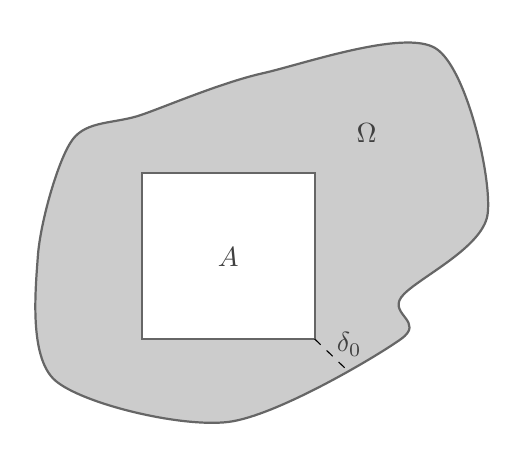
\begin{tikzpicture}
			 \begin{axis}[axis x line=none, axis y line=none]
				\addplot[mark=none, black!60, smooth cycle, thick, fill=gray!40] coordinates {(1,1) (2,0.5) (3,1.5) (3,2) (3.5,3) (3.2, 5) (2.2, 4.7) (1.5, 4.2) (1.1, 3.9) (0.9, 2.5)};
				\node[black!75] at (axis cs:2.8,3.75) [anchor=south] {$\Omega$};
				\addplot[mark=none, black!60, thick, fill=white!30] coordinates {(2.5,1.5) (2.5,3.5) (1.5,3.5) (1.5,1.5) (2.5,1.5)};
				\node[black!75] at (axis cs:2,2.25) [anchor=south] {$A$};
				\addplot[dashed] coordinates {(2.5,1.5) (2.7,1.1)};
				\node[black!75] at (axis cs:2.7,1.175) [anchor=south] {$\delta_{0}$};
			 \end{axis}
			\end{tikzpicture}
		\end{figure}
			
		Da $\supp(\phi_{\delta}) \subset B(0, \delta)$ nach \hyperref[bem:8.7ii]{8.7 ii)}
		\[ \Rightarrow \supp(g \ast \phi_{\delta} ) \subset A + B\left(0, \frac{\delta_{0}}{2}\right) \subset \Omega \text{ für } \delta < \frac{\delta_{0}}{2} \]
		(mit $A + B \coloneqq \{ x + y : x \in A, y \in B\}$), denn $g \ast \phi_{\delta}(u) = \int \phi_{\delta}(u - v) g(v) dv \neq 0$ nur wenn $v \in A$ und $\| u - v \| < \delta$. \\
		Also $g \ast \phi_{\delta} \in C_{c}(\Omega)$. Zu zeigen: $g \ast \phi_{\delta} \in C^{\infty}(\Omega)$
		\[ D_{u}^{\alpha}(\phi_{\delta} \ast g)(u) = \int_{A} \left[ D_{u}^{\alpha} \phi_{\delta}(u - v) \right] \underbrace{g(v)}_{\text{beschränkt}} gv \]
		d.h. $\phi_{\delta} \ast g \in C	^{\infty}$; in einfachen Worten bedeutet das, dass $C_{\delta} \ast g$ alle guten Eigenschaften von $\phi$ $"$erbt$"$, auch wenn $g$ $"$schlecht$"$ ist. \\
		\[ \| f - \phi_{\delta} \ast g \|_{L^{p}} \leq \underbrace{\| f - g \|}_{\leq \epsilon} + \underbrace{\| g - \phi_{\delta} \ast g \|_{L^{p}}}_{\leq \epsilon} \text{ für } \epsilon \text{ klein genug nach } \hyperref[satz:8.8]{8.8} \]
	\end{beweis}
\end{kor}


\begin{bemerkung*}
	Es gilt:
	\begin{itemize}
		\item $\supp(f) \subset A, \supp(g) \subset B \quad \Rightarrow  \quad \supp(f + g) \subset A + B $
		\item $f \ast g = g \ast f$
	\end{itemize}	
\end{bemerkung*}


\begin{kor} \label{kor:8.10}
	Sei $\Omega \subseteq \MdR^{d}$ offen. Sei $f \in L^{p}(\Omega), p \in [1, \infty)$ mit $\int f(u) g(u) du = 0$ für alle $g \in C_{c}^{\infty}(\Omega)$. Dann ist $f = 0$.
	\begin{beweis}
		Zu $f \in L^{p}$ gibt es ein $g \in L^{p'}, \frac{1}{p} + \frac{1}{p'} = 1$ mit 
		\[ \| f \|_{L^{p}} = \int f(u) g(u) du, \quad \| g \|_{L^{p'}} = 1 \]
		Wähle $g(u) = |f(u)|^{p - 1} \left( sign(f(u)) \right) \cdot \| f \|_{L^{p}}^{\frac{1}{p} - 1}$. Dann ist
		\begin{align*}
			\| f \|_{L^{p}} & = \left( \int |f(u)|^{p} du \right)^{\frac{1}{p}} = \| f \|_{L^{p}}^{\frac{1}{p} - 1} \int |f(u)|^{p} du \\
			& = \int f(u) \underbrace{\frac{sign(f(u)) |f(u)|^{p - 1}}{\| f \|^{1 - \frac{1}{p}}}}_{=: g(u)} du \\
			& = \int f(u) g(u) du
		\end{align*}
		$\| g \|_{L^{p'}} = 1$ mit $\frac{1}{p} + \frac{1}{p'} = 1$. (sieh auch \hyperref[satz:8.1]{Beweis 8.1}) 
		\[ \| f \|_{L^{p}} = \int f(u) g(u) du = \int f(u) [g(u) - \phi(u)] du \text{ für alle } \phi \in C_{c}^{\infty}(\Omega), \quad \text{ denn } \int f(u) \phi(u) du = 0 \]
		Wähle nach \hyperref[kor:8.9]{8.9} ein $\phi \in C_{c}^{\infty}(\Omega)$ mit $\| g - \phi \|_{L^{p'}(\Omega)} < \frac{1}{2}$ \\ \\
		Also $\| f \|_{L^{p}} \underset{\text{Hölder}}{\leq} \| f \|_{L^{p}} \| f - \phi \|_{L^{p'}} < \frac{1}{2} \| f \|_{L^{p}}$, was einen Widerspruch zu $f \neq 0$ darstellt, demnach gilt $\| f \|_{L^{p}} = 0, f = 0$.
	\end{beweis}
\end{kor}



\newpage		
	
	\section*{Elem. der Op.Theo.}	
		\subsection*{9 - Baire \& B.-S.}

	\begin{karte}{Satz von Baire}
		Sei $(M, d)$ ein vollständiger metrischer Raum und seien $(U_{n})_{n \geq 1}$ offen und dicht in $M$.
		\[ \text{Dann ist } \bigcap_{n \in \MdN} U_{n} \text{ dicht in } M. \]
	\end{karte}
	
	
	\begin{karte}{nirgends dicht}
		Eine Teilmenge $L$ eines metrischen Raums $M$ hei{\ss}t \begriff{nirgends dicht}, falls $\overline{L}$ keine inneren Punkte enthält.
		
		Ist $L$ nirgends dicht, dann ist $M \setminus \overline{L}$ dicht in $M$.	
	\end{karte}

	\begin{karte}{1. Kategorie}
		Eine Teilmenge $L$, die sich als Vereinigung von einer Folge von nirgends dichten Mengen $L_{n}$ darstellen lässt, d.h. $L = \bigcup_{n \in \MdN} L_{n}$ hei{\ss}t von \begriff{1. Kategorie}.		
	\end{karte}

	\begin{karte}{2. Kategorie}
		$L$ hei{\ss}t von \begriff{2. Kategorie}, falls $L$ nicht von 1. Kategorie ist.		
	\end{karte}
	
	\begin{karte}{Kategoriensatz von Baire}
		\begin{enumerate}[label=\alph*\upshape)]
			\item In einem vollständigen metrischen Raum $(M, d)$ liegt das Komplement einer Menge $L$ von 1. Kategorie stets dicht. Insbesondere:
			\item Ein vollständig metrischer Raum ist von 2. Kategorie
			\item Sei $(M, d)$ vollständig und $(M_{n})_{n \geq 1}$ eine Folge abgeschlossener Mengen mit $M = \bigcup_{n \in \MdN} M_{n}$. Dann enthält mindestens ein $M_{n}$ eine Kugel
		\end{enumerate}	
	\end{karte}

	\begin{karte}{Dichte Teilmenge von $(C[0, 1], \|\cdot\|_{\infty})$}	
		$E = \{ x \in C[0, 1]:$ $x$ ist in keinem Punkt von $[0, 1]$ differenzierbar$\}$ ist dicht in $(C[0, 1], \|\cdot\|_{\infty})$. \\
		Insbesondere:
 		\begin{itemize}
			\item $E \neq \emptyset$
			\item $C^{1}[0, 1]$ ist von 1. Kategorie in $C[0, 1]$, also liegt $C[0, 1] \setminus C^{1}[0, 1]$ dicht in $C[0, 1]$.
		\end{itemize}
	\end{karte}
	
	\begin{karte}{Banach-Steinhaus}
		Sei $X$ ein Banachraum, $Y$ ein normierter Raum, $I$ eine Indexmenge und $(T_{i})_{i \geq 1} \in B(X, Y)$.
		Falls:
		\[ \sup_{i \in I} \| T_{i} x \| = c(x) < \infty, \quad \forall x \in X \]
		dann ist auch
		\[ \sup_{i \in I} \| T_{i} \| = \sup_{i \in I} \sup_{\| x \| \leq 1} \| T_{i} x \| < \infty. \]
	\end{karte}			
		\subsection*{10 - offenen Abbildung}

	\begin{karte}{Offene Abbildung}
			Eine Abbildung zwischen metrischen Räumen heißt \begriff{offen}, wenn offene Mengen auf offene Mengen abgebildet werden.
	\end{karte}
	
	\begin{karte}{Äquivalenzen zu offenem Operator}
				Seien $X, Y$ normierte Räume und $T: X \rightarrow Y$ ein linearer Operator, dann sind äquivalent:
		\begin{enumerate}[label=\alph*\upshape)]
			\item $T$ ist offen
			\item $\exists \epsilon > 0: K_{Y}(0, \epsilon) \subset T(K_{X}(0, 1))$
		\end{enumerate}
	\end{karte}
	
	\begin{karte}{Satz von der offenen Abbildung}
		Seien $X, Y$ Banachräume und $T \in B(X, Y)$, dann gilt:
		\[ T \text{ surjektiv} \gdw T \text{ offen} \]
	\end{karte}

	\begin{karte}{Bijektiver beschränkter Operator}	
		Seien $X, Y$ Banachräume und $T \in B(X, Y)$ bijektv, dann ist $T^{-1} \in B(Y, X)$	
	\end{karte}

	\begin{karte}{Beschränkte Einbettung zwischen Banachräumen}	
		Sei $X$	ein Vektorraum der sowohl mit $\| \cdot \|$ als auch mit $\vertiii{\cdot}$ ein Banachraum ist. Gilt 
		\[ \exists c > 0: \| x \| \leq c \cdot \vertiii{x}, ~ \forall x \in X, \]
		dann sind die Normen äquivalent, d.h. $\exists \hat{c} $ mit $\hat{c} \cdot \vertiii{x} \leq \| x \|$ $\forall x \in X \leq c \cdot \vertiii{x}$. 
	\end{karte}
		\subsection*{11 - Projektionen}

	\begin{karte}{Projektion, \\ und die Existenz der Einbettung in Untervektorraum}
	Sei $X$ ein Banachraum. $P \colon X \rightarrow X$ hei{\ss}t \begriff{Projektion}, wenn $P$ linear und $P^{2} = P$ ist. \\


	Sei $X$ ein Vektorraum, $M \subset X$ ein Untervektorraum. Es gibt nach dem Basisergänzungssatz eine lineare Projektion 
		\[ P \colon X \rightarrow X, P(X) = M \]	
	\end{karte}

	\begin{karte}{Direkte Summe von Banachräumen}
	Sind $X, Y$ Banachräume, dann ist auch $X \oplus Y$ ein Banachraum mit $\| (x, y) \|_{X \bigoplus Y} = \| x \|_{X} + \| y \|_{Y}$ $\forall x \in X, y \in Y$
	\end{karte}

	\begin{karte}{Äquivalenzen zur Existenz einer stetigen Projektion auf Untervektorraum}
	Sei $X$ ein BR, $M \subset X$ ein abg. UVR. Dann sind äquivalent:
	\begin{enumerate}[label=\alph*\upshape)]
		\item $\exists$ stetige Projektion $P \colon X \rightarrow X$, $P(X) = M$
		\item Es gibt einen abg. UVR $N \subset X: X = M \oplus N$.
		\item $\exists$ abg. Untervekottraum $N \subset X$ und $J: M \oplus N \rightarrow X,$ $J(x, y) = x + y$ ist ein Isomorphismus, insbesondere $\exists c > 0$ $\forall x \in M, y \in N:$ $c \left( \|x \| + \|y \| \right) \leq \|x + y \| \leq \|x \| + \| y \| $
	\end{enumerate}
	$M$ hei{\ss}t komplementierter Raum, \\
	$N = \kernn(P)$ Komplementärraum.
	\end{karte}
		\subsection*{12 - Abg. Operatoren}

	\begin{karte}{Operatorfortsetzung}
		Sei $X$ ein Banachraum, $D(A)$ ein dichter Untervektorraum und $A: D(A) \rightarrow X$ linear
	
		Gilt $\| A x \| \leq c \| x \|$ $\forall x \in D(A)$, so lässt sich $A$ zu einem beschränkten Operator fortsetzen $A \in B(X)$	
	\end{karte}
	


	\begin{karte}{Graphennorm}
		Auf $D(A)$ definieren wir die \begriff{Graphennorm}
		\[ \| x \|_{A} \coloneqq \|x \| + \| A \| \quad \forall x \in D \]
		Insbesondere: $A: (D(A), \| \cdot \|_{A}) \rightarrow X$ stetig, denn 
		\[ \| X \| \leq \|x \| + \| A x \| = \| x \|_{A} \]
	\end{karte}


	\begin{karte}{Abgeschlossener Operator}
		Es sind äquivalent
		\begin{enumerate}[label=\alph*\upshape)]
			\item $\left( D(A), \| \cdot \|_{A} \right)$ ist ein Banachraum
			\item $\ograph(A) = \{ (x, A x): x \in D(A) \} \subset X \times X$ ist abgeschlossen
			\item Wenn $(x_{n})_{n} \subset D(A): \begin{cases}
			x_{n} \xrightarrow[]{n \rightarrow \infty} x & \text{ in } X \\ A x_{n} \xrightarrow[]{n \rightarrow \infty} y & \text{ in } X \end{cases}$, $ $ so ist $x \in D(A), A x = y$
		\end{enumerate}
	
		$A$ hei{\ss}t abgeschlossen, wenn $a) - c)$ aus \hyperref[satz:12.3]{12.3} erfüllt sind	
	\end{karte}


	\begin{karte}{Abgeschlossener vs. stetiger Operator}
		\begin{align*}
			A \text{ stetig: } & x_{n} \xrightarrow[]{n \rightarrow \infty} x \Rightarrow Ax_{} \xrightarrow[]{n \rightarrow \infty} y, Ax = y \\
			A \text{ abgeschlossen: } & x_{n} \xrightarrow[]{n \rightarrow \infty} x, A x_{n} \xrightarrow[]{n \rightarrow \infty} y \Rightarrow Ax = y
		\end{align*}
	\end{karte}


	\begin{karte}{Satz vom abgeschlossenen Graphen}
		Ist $A$ abgeschlossen und $D(A) = X$, so ist $A$ stetig auf $X$.
	\end{karte}

		
\end{document}